% Chapter 5

\chapter{Discovering Event-specific Informative Content from Twitter} % Main chapter title

\label{TwitterStudy} % For referencing the chapter elsewhere, use \ref{Chapter1} 

\lhead{Chapter 5. \emph{Discovering Event-specific Informative Content from Twitter}} % This is for the header on each page - perhaps a shortened title

Twitter has brought a paradigm shift in the way we produce and curate information about real-life events. Huge volumes of user-generated tweets are produced in Twitter, related to events. Not, all of them are useful and informative. A sizable amount of tweets are spams and colloquial personal status updates, which does not provide any useful information about an event.  Thus, it is necessary to identify, rank and segregate event-specific informative content from the tweet streams. In this chapter, we implement \textit{EventIdentityInfoGraph} and \textit{EventIdentityInfoRank} as introduced in \ref{EventIdentityInformationProcessing} in the context of Twitter. We name \textit{EventIdentityInfoGraph} as \textit{TwitterEventInfoGraph} and \textit{EventIdentityInfoRank} as \textit{TwitterEventInfoRank}. Mutually reinforcing relationships between tweets, hashtags, text units, URLs and users are defined and represented using \textit{TwitterEventInfoGraph}. \textit{TwitterEventInfoRank} simultaneously ranks tweets, hashtags, text units, URLs and users in terms of event-specific informativeness by leveraging the semantics of relationships between each of them as represented by \textit{TwitterEventInfoGraph}. Experiments and observations are reported on four million (approx) tweets collected for five real-life events, and evaluated against popular baseline techniques showing significant improvement in performance. 

\section{Twitter and Event Related Content}

\noindent Social media platforms provide multiple venues to people for sharing first-hand experiences and exchange information about real-life events. Twitter is one such platform that has become an indispensable source for disseminating news and real-time information about current events. It is a microblogging application that allows its users to post short messages of 140 characters known as tweets, from a variety of internet enabled devices. Studies have shown the importance of Twitter as a news circulation service \cite{phelan2009using}, and a source for gauging public interest and opinions \cite{o2010tweets}. It's efficacy as a real-time citizen-journalistic source of information has been recently harnessed in detection, extraction and analysis of real-life events \cite{sakaki2013tweet,popescu2011extracting,purohit2013twitris}.

 

%Table \ref{tweetsample} presents few examples of informative and uninformative tweets.  In this work we consider tweets having news worthy content, recent updates and real-time coverage of on-going events, that are suitable for general audience, as informative.

\begin{table}[htbp]
\centering
\caption{Examples of different event related tweets.}
\label{tweetsample}
     \begin{tabular}{|p{14cm}|} \hline
     Ted Cruz is a dangerous man. Crazy and gaining support. Megalomaniac leaders are bad, mkay. \#CPAC \#politics \#joke [\textit{\textbf{personal/uninformative}}] \small \textit{\textbf{Event: `CPAC 2014'}}\\ \hline
     Thanks for the memories Sochi! I've had the time of my life \#Sochi2014 \#sochiselfie http://t.co/DqkLEaAMpo. [\textit{\textbf{personal/uninformative}}] \small \textit{\textbf{Event: `Sochi Games'}} \\ \hline
     \#SXSW14 \#SXSW \#sxswinteractive \#CPAC2014 \#CPAC \#CPACPickupLines \#CPACPanels Be squared away \@ perky TOP TWEETED of http://t.co/h0igdOVNW0. [\textit{\textbf{spam/uninformative}}] \small \textit{\textbf{Event: `CPAC 2014'}}\\ \hline
In \#Sochi, the Dutch are dominating the overall Olympic medal count http://t.co/jMR1WUqEK4 (Reuters) http://t.co/dAfDhEgTGA. [\textit{\textbf{event-specific informative}}] \small \textit{\textbf{Event: `Sochi Games'}}\\ \hline
New post: Sochi Was For Suckers - Laugh Studios/ http://t.co/cWQJCBp3Ow \#lol \#funny \#rofl \#funnypic \#fail \#wtf. [\textit{\textbf{spam/uninformative}}] \small \textit{\textbf{Event: `Sochi Games'}}\\ \hline
It's \@tedcruz vs. \@SenJohnMcCain in a \#CPAC spat. What did they say? Find out on \#AC360 8p on \@CNN. [\textit{\textbf{event-specific informative}}] \small \textit{\textbf{Event: `CPAC 2014'}} \\ \hline
     \end{tabular}
\end{table}

Users not only post plain textual content in their messages but also share URLs, linking to other external websites, images and videos. Apart from creating new content, the users also share content produced by others. This activity is known as \textit{retweeting}, and such tweets are preceded by special characters `\textit{RT}'. The messages are normally written by a single person and are read by many. The readers in this context are known as \textit{followers}, and the user whom they follow is considered as their \textit{friend}. Any user with good intent either share messages 
that might be of interest to his followers, or for joining conversations on topics of his interest. The `@' symbol followed by the username commonly known as \textit{user mentions}, is used for mentioning other users in tweets for initiating conversations. 

The concise and informal content of a tweet is often contextualized by the use of a crowdsourced annotation scheme called \textit{hashtags}. Hashtags are a sequence of characters in any language prefixed by the symbol `\#' (for e.g. \#websci2015). They are widely used
by the users for categorizing the content based on a topic, join conversations related to a topic, and to make the tweets easily searchable by other interested users. They also act as strong identifiers of topics \cite{laniado2010making}. When tweeting about real-life events the users also tend to use hashtags in order to post event-specific content. For e.g. `\#Egypt' and `\#Jan25', were among the most popular hashtags in Twitter used for spreading, organizing and analyzing information related to `Egyptian Revolution of 2011' \cite{barrons2012suleiman}. 


284 million monthly users of Twitter posting 500 million tweets per day produces a variety of content\footnote{\tiny http://about.twitter.com/company}. A significant proportion of it are related to different real-life events (e.g, football matches, conferences, music shows, etc). Majority of this content are personal updates (e.g.  \textit{Thanks for the memories Sochi! I've had the time of my life \#Sochi2014 \#sochiselfie http://t.co/DqkLEaAMpo}), pointless babbles (e.g. \textit{Ted Cruz is a dangerous man. Crazy and gaining support. Megalomaniac leaders are bad, mkay. \#CPAC \#politics \#joke}) and spams (e.g \textit{New post: Sochi Was For Suckers - Laugh Studios/ http://t.co/cWQJCBp3Ow \#lol \#funny \#rofl \#funnypic \#wtf.}). Personal views and conversations might be of interest to a specific group of people. However, they are meaningless and provides no information to the general audience. On the other hand there are tweets that presents newsworthy content, recent updates and real-time coverage of on-going events (e.g. \textit{In \#Sochi, the Dutch are dominating the overall Olympic medal count http://t.co/jMR1WUqEK4 (Reuters) http://t.co/dAfDhEgTGA}). These tweets provide event-specific informative content and are more useful for general audience interested to know about the event. We call them as event-specific informative tweets. Table \ref{tweetsample} presents some examples of different types of tweets shared during real-life events.

\section{Motivation} 
With the plethora of event related content being produced in Twitter, it becomes inconvenient for users to search and follow informative posts. This necessitates development of techniques that can identify and rank tweets in terms of their event-specific informativeness. In addition to the tweets, a backend automated system dedicated for processing, analyzing and presenting information from Twitter during an event, could get immensely benefitted from identification and ranking of event-specific informative hashtags, text units, users and URLs. This would enable the system to generate answers to questions like:
\begin{itemize}
\item \textit{Who are the users producing large amount of event-specific informative content?}
\item \textit{Which are the best hashtags and URLs to follow that would lead to high quality event-specific information?}
\item \textit{Which are the best hashtags and text units to index for efficient retrieval of event-specific information?}
\item \textit{Which are the most informative tweets sharing event-specific information?}
\end{itemize}
Such a system would further facilitate better consumption of content while exploring event information from Twitter. It could have a positive impact on triggering event-specific recommendations and efficient processing of information. It can act as a core component of event management, event summarization, event marketing and journalistic platforms leveraging Twitter.


\section{Challenges in Mining Tweets} 
\subsection{Information Overload affecting Consumption and Collection of Data}
As already pointed out previously that Twitter produces 500 million posts per day, that is distributed across its 288 million active users. This huge amount of content being generated increases the chances of an user to experience an overload of information that is left for him to consume. Surveys show that two thirds of Twitter users have felt that they receive too many posts, and over half of Twitter users have felt the need for a tool to filter out the irrelevant posts \cite{bontcheva2013social}. \cite{rodriguez2014quantifying} also attempted to study and quantify information overload experienced by users in Twitter.

Due to the large volumes of information that needs to be stored and processed by Twitter on a daily basis, it also becomes a challenging job to build a infrastructure that can handle queries and information seeking needs of its millions of users. Therefore, the API endpoints provided by Twitter for collecting live data, results in collection of a biased sample. The Twitter Streaming API provides only a random sample of 1\%  of the total public stream produced in real-time, also known as spritzer sample. For accessing larger samples one needs to subscribe to Firehose services that are often costly and are seldom used by the researchers in an academic setting.

\subsection{Idiosyncratic Structure and Informal Language}
Unlike news documents and blogs, tweets pose additional challenges in the tasks of summarization, information retrieval, topic detection, entity extraction and POS tagging, due to the colloquial language used and limitation of 140 characters forcing the users to express the content in unusual grammatical structures that are not common in other publishing websites. The state-of-the-art entity extraction techniques depend on local linguistic features, common in well-formed documents like capitalization and POS tags of previous words \cite{ratinov2009design}. Such characteristics is uncommon in tweets due to extensive use of informal language. Limitation in length, extensive and unusual usage of abbreviations, capitalization and uncommon grammar makes it extremely difficult for the text mining techniques to identify valuable and useful content \cite{bontcheva2013twitie}. Due to live conversations between the users during real-life events it is also difficult to extract event related information as the conversation tweets often lack context. Intentional misspellings sometimes demonstrate examples of intonation in written text \cite{prevost1996information}. For instance, expressions like, `this is so cooool', emphasizes stress on the emotions and conveys more information that should be captured. It has been shown that it is extremely challenging for the state-of-the art information extraction algorithms to perform efficiently and give accurate results for micro-blogs \cite{derczynski2013microblog}. For example, named entity recognition methods typically show 85-90\% accuracy on longer texts, but 30-50\% on tweets \cite{ritter2011named}.





\subsection{Nepotistic relationships}

\subsection{Data Management Challenges}



\section{Objective and Contributions} The main objective of the work presented in this chapter is to automatically identify and rank event-specific informative content posted in Twitter. Our primary hypothesis is that there are explicit cues available in the content of the tweets posted during an event for determining event-specific informativeness. Our approach is based on the \textit{principle of mutual reinforcement} commonly used for summarization of textual documents. We build our methodology on the basic tenets of \textit{Mutually Reinforcing Chains} \cite{wei2008query}, for ranking and identification of event-specific informative content in Twitter. We make the following contributions:



%towards analysis, representation and identification of informative content in Twitter, related to events:
\begin{itemize}
%\item analyze the characteristics of informative and non-informative content in event related tweets;
\item analysis of informative and non-informative content in 3.8 million event related tweets;
\item propose a generic model based on principle of mutual reinforcement that takes into account the semantics of relationships between \textit{tweets}, \textit{hashtags}, \textit{text units}, \textit{URLs} and \textit{users}, and represent them in a graph structure - \textit{TwitterEventInfoGraph};
\item leverage the mutually reinforcing relationships in \textit{TwitterEventInfoGraph} and develop a graph based iterative algorithm - \textit{TwitterEventInfoRank}, for simultaneously ranking \textit{tweets}, \textit{hashtags}, \textit{text units}, \textit{users} and \textit{URLs} in terms of event-specific informativeness;
\item evaluate the algorithm against popular baselines and report its performance in identifying and ranking event-specific informative content from Twitter.
\end{itemize}



\section{Analysis of Event Related Tweet Content\label{analysis}}

%Twitter allows its users to post short messages with a limitation of 140 characters. Users not only post plain textual content in their messages but also share urls, linking to other external websites, images and videos. The images and videos are 
%labeled as media elements by Twitter. Apart from curating new content, the users also share content produced by others. This activity is known as \textit{retweeting}, and such tweets are preceded by the special characters \textit{RT}.
%The messages are normally written by a single person and are read by many. The readers in the context of Twitter are known as \textit{followers}, and the user whom the other users follow is considered as their \textit{friend}. Any user with good intent either share messages 
%that might be of interest to his followers, or for joining conversations on topics of his interest. The `@' symbol followed by the username commonly known as \textit{user mentions}, is used for mentioning other users in tweets for initiating conversation with them. 
%
%The concise and informal content of a tweet is often contextualized by the use of a crowdsourced annotation scheme called \textit{hashtags}. Hashtags are a sequence of characters in any language prefixed by the symbol `\#' (for e.g. \#icwsm2015). They are widely used
%by the users in order to add context to the tweets, categorizing the content based on a topic, join conversations related to a topic, and to make the tweets easily searchable by other interested users. They also act as strong identifiers of topics \cite{laniado2010}. When tweeting about real-life
%events the users also tend to use hashtags in order to post event-specific content. For example `\#Egypt' and `\#Jan25', were among the most popular hashtags in Twitter used for spreading, organizing and analyzing information related to `Egyptian Revolution of 2011' \cite{barrons2012}. 
%The widespread use of hashtags for labeling event related tweets has also led to the coining of the term, \textit{hashtag activism}.

\begin{table}[htbp]
\center
\caption{Details of data collected for analyzing event related tweet content.}
\label{informationcuedata}
\begin{tabular}{|c|c|c|}
\hline
\shortstack{\textbf{Event Name and} \\ \textbf{Query Hashtag}}                            & \shortstack{\textbf{No. of} \\ \textbf{Tweets}} & \shortstack{\textbf{Time Period}}                               \\ \hline
\shortstack{Sochi Winter\\ Games 2014 \\ (\#sochi2014) \\ ($http://goo.gl/sG4Rqd$)} & 1958220 & \shortstack{11th Feb,2014\\ to\\ 3rd March, 2014} \\ \hline
%\begin{tabular}[c]{@{}c@{}}Millions March \\ NYC\\ (\#millionsmarchnyc)\end{tabular}                    & 56927                                                             & \begin{tabular}[c]{@{}c@{}}13th Dec, 2014\\ 20:25:43\\ to\\ 14th Dec, 2014\\ 03:30:41\end{tabular} \\ \hline
\begin{tabular}[c]{@{}c@{}}SXSW 2014 \\ (\#sxsw2014) \\ ($http://goo.gl/b6Nd6X$)\end{tabular}                                  & 1880557                                                            & \begin{tabular}[c]{@{}c@{}}8th March, 2014\\ to\\ 16th March, 2014\end{tabular} \\ \hline
\begin{tabular}[c]{@{}c@{}}CPAC 2014 \\ (\#cpac2014) \\ ($http://goo.gl/9o1KUx$)\end{tabular} & 18104                                                              & \begin{tabular}[c]{@{}c@{}}7th March, 2014\\ to\\ 16th March, 2014\end{tabular} \\ \hline
\end{tabular}
\end{table}

Given the mechanisms of user interactions and content production  in Twitter as explained in Section 1, we analysed 3.8 million (approx) English tweets produced during three real-life events. Details of the data related to the events, collected for conducting the analysis is presented in Table \ref{informationcuedata}\footnote{\tiny Note: This dataset is different from the dataset that we use for our experiment and evaluation. Refer Section 6.1 for the reason.}. We provided a popular hashtag corresponding to each event to the Twitter streaming API\footnote{\tiny https://dev.twitter.com/streaming/overview} in order to collect the data over the indicated period of time. The text of the tweets were preprocessed and prepared for analysis (Refer Section \ref{dataprep} for details). One of the main intentions behind this analysis was to investigate the nature of content in informative and non-informative tweets and to understand if there is a difference between tweets rich in generic information and the ones with event-specific information. 
%The analysis was done for building an intuition about the cues that aids in detecting informative content. We use the cues for identifying event-specific \textit{ information units} and relationships between them in event related tweets. This is further used in building a generic framework for identifying and ranking event-specific informative tweets. 

%Conversation in Twitter by mentioning other users in the tweets might be done in a personal context.  It is less likely that these conversations would convey information suitable for a general audience. 

%We started our analysis with the assumption that the content of a tweet is primarily composed of hashtags, words for expressing and conveying information, and urls that lead to additional information about the content. We plotted the distribution of occurrences of all the hashtags, tokens and shared urls for each event. Due to the short length of the tweets we only considered unigram tokens. We also plotted the distribution of the number of tweets posted by the users.
%We observed a power law distribution for all of them (refer Figure \ref{fg:figure3}). This gave us an intuition that there are skewed sets of hashtags and tokens that are widely used for posting content related to an event. 
%%We call them \textit{event-specific hashtags} and \textit{event-specific text units}. 
%There is also a specific set of urls that become popular in comparison to others and a set of users who are more active than others in posting event related content. 
%We call them \textit{event-specific urls} and \textit{event-specific users}, respectively. 




\begin{savenotes}
\begin{table}[ht]
\centering
\caption{Tweet features for content informativeness.}
\label{tweetfeature}
\begin{tabular}{|l|}
\hline
Has Url, No. of words, No. of stopwords, No. of feeling words, No. of slang \\ 
words, No. of hashtags, No. of user mentions, Tweet  length (No. of characters),\\  No. of unique 
characters, No. of special characters, Favorite count, Retweet \\ count, Formality, Is tweet verified, No. of nouns, No. of adjectives, No. of \\ verbs, No. of adverbs, No. of pronouns, No. of interjections, No. of articles, \\ No. of prepositions.
 \\ \hline
\end{tabular}
\end{table}
\end{savenotes}

\begin{table}[ht]
\centering
\caption{Evaluation measures for logistic regression model.}
\label{logregreseval}
\begin{tabular}{c|c|c|c|}
\cline{2-4}
\multicolumn{1}{l|}{}                          & \textbf{Precision} & \textbf{Recall}       & \textbf{F1-score}     \\ \hline
\multicolumn{1}{|c|}{\textbf{Non-informative} (0)} & 0.70               & 0.49                  & 0.57                  \\ \hline
\multicolumn{1}{|c|}{\textbf{Informative} (1)}     & 0.78               & 0.90                  & 0.84                  \\ \hline
\multicolumn{1}{|c|}{\textbf{Avg/Total}}       & 0.76               & 0.77                  & 0.75                  \\ \hline
\multicolumn{1}{|c}{\textbf{Accuracy}} =  & \multicolumn{1}{l}{} 76.64\%            & \multicolumn{1}{l}{} & \multicolumn{1}{l|}{} \\ \hline
\end{tabular}
\end{table}

\begin{figure}[htbp]
\centering
\caption{Content characteristics of informative and non-informative tweets related to events.}
    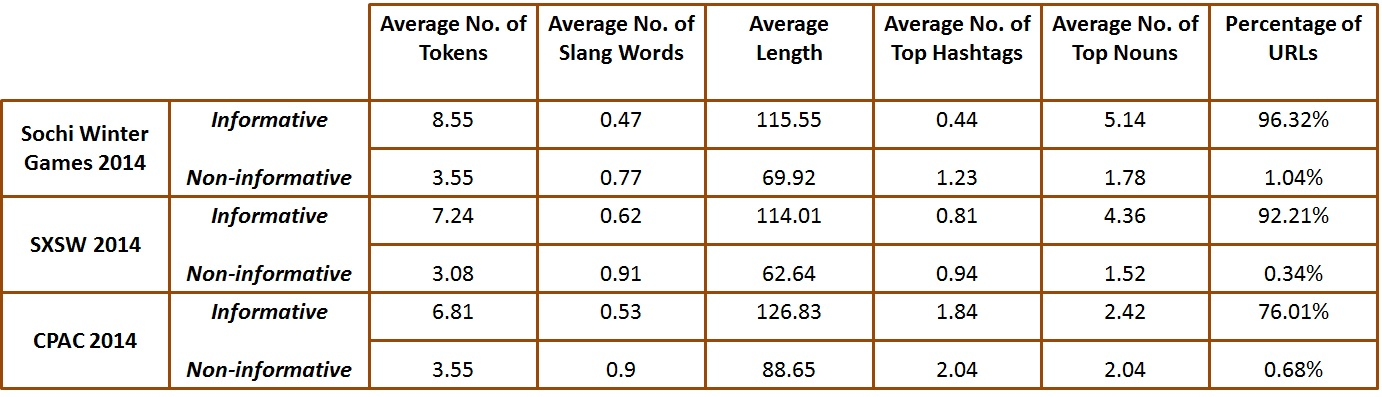
\includegraphics[width=15cm,height=5.5cm]{Figures/InformationAnalysisTable.jpg}
    
    \label{infoanalysis}
\end{figure}

%\begin{table*}
%\centering
%\caption{Content characteristics of informative and non-informative tweets related to events.}
%\label{tweetcharacteristics}
%\begin{tabular}{c c|c|c|c|c|c|c|}
%\cline{3-7}
%& & \multicolumn{5}{ c| }{\textbf{Average content characteristics per tweet}} \\ \cline{3-7}
%\cline{3-8}
%& & \textbf{\# of words} & \textbf{\# of slang words} & \textbf{Length} & \textbf{Top hashtags} & \textbf{Top nouns} & \textbf{Urls Percent} \\ \cline{1-8}
%\multicolumn{1}{ |p{1.8cm} }{\multirow{2}{*}{\shortstack{\textbf{Sochi Winter} \\ \textbf{Games 2014}}} } &
%\multicolumn{1}{ |c|}{\textbf{\textit{Informative}}} &  8.55 & 0.47 & 115.55 & 0.44 & 5.14 & 96.32\%  \\ \cline{2-8}
%\multicolumn{1}{ |c }{}                        &
%\multicolumn{1}{ |c| }{\textbf{\textit{Non-informative}}} & 3.55 & 0.77 & 69.92 & 1.23 & 1.78 &  1.04\%  \\ \cline{1-8}
%\multicolumn{1}{ |p{1.8cm}  }{\multirow{2}{*}{\textbf{SXSW 2014}} } &
%\multicolumn{1}{ |c| }{\textbf{\textit{Informative}}} & 7.24 & 0.62 & 114.01 & 0.81 & 4.36  & 92.21\% \\ \cline{2-8}
%\multicolumn{1}{ |c  }{}                        &
%\multicolumn{1}{ |c| }{\textbf{\textit{Non-informative}}} & 3.08 & 0.91 & 62.64 & 0.94 & 1.52 & 0.34\%  \\ \cline{1-8}
%\multicolumn{1}{ |p{1.8cm}  }{\multirow{2}{*}{\textbf{CPAC 2014}} } &
%\multicolumn{1}{ |c| }{\textbf{\textit{Informative}}} & 6.81 & 0.53 & 126.83 & 1.84 & 2.42 & 76.01\% \\ \cline{2-8}
%\multicolumn{1}{ |c  }{}                        &
%\multicolumn{1}{ |c| }{\textbf{\textit{Non-informative}}} & 3.55 & 0.9 & 88.65 & 2.04 &  1.0 & 0.68\% \\ \cline{1-8}
%
%\end{tabular}
%\end{table*}

\subsection{Analysis of Informative and Non-informative Content in Tweets} Our first step was to segregate the tweets likely to have informative content from the non-informative ones. In order to do so we trained a logistic regression model on an annotated dataset \cite{olteanu2014crisislex}, which is publicly available. 9729 English language annotated tweets were used for building the model. The tweets labeled as \textit{related and informative} were assigned a score of 1 and all the other tweets labeled as \textit{related - but not informative} and \textit{not related} were assigned a score of 0. Table \ref{tweetfeature} lists the features selected for each tweet. The choice of the features
was driven by previous studies pointed out in Section 2. 10-fold cross validation was performed resulting in a model with an accuracy of 76.64\%. Refer Table \ref{logregreseval} for evaluation measures.

\begin{align*}
Formality = (No.\, of \, nouns + No.\, of \,adjectives + No. \,of\, prepositions + No.\, of\, articles \\ 
-  No.\, of\, pronouns - No.\, of\, verbs - No.\, of\, adverbs - No.\, of\, interjections + 100)/2
\end{align*}


The logistic regression model was then used for assigning informativeness score between 0 and 1 to all the tweets in the dataset, with 0 being least informative and 1 being most informative. Although, the model is developed on tweets related to disaster events, it has been shown by the 
authors \cite{Imran2013} that the annotations could be generalized to any type of event. The tweets for each event were then separated into two subsets - \textit{informative}, containing
tweets scoring more than 0.7, and \textit{non-informative}, containing tweets scoring less than 0.3. Average values of  different content characteristics of tweets were calculated for both the subsets. The top 10\% of the frequently occurring hashtags, nouns and URLs were considered as top hashtags, nouns and URLs for the analysis, respectively. Some of the characteristics that were noticeably different for informative and
non-informative tweets are listed in Table \ref{tweetcharacteristics}.
%of few properties important for determining informativeness based on our intuition are listed in Table \ref{tweetcharacteristics}.

For all the events, on an average, the informative tweets were marked by a higher number of words per tweet and greater occurrence of top nouns. The average length of informative tweets were also more than the non-informative ones. The percentage of informative tweets having URLs were strikingly high. As expected, a greater usage of slang words was observed in non-informative tweets. However, the greater occurrence of top hashtags in non-informative tweets urged us to look into the content. We found that a lot of non-informative tweets have used many popular hashtags with unrelated content and URLs pointing to irrelevant information. This is typical of spam tweets as already reported by \cite{yardi2009detecting}. Not shown due to space constraints, a larger average occurrence of feeling words and top URLs was observed in informative tweets. The average number of follower counts for users posting informative tweets was also observed to be higher than the ones posting non-informative ones.

The above observations gave us an idea of how informative content about events is generally produced in Twitter and the characteristics that differentiates it from non-informative ones. It is now intuitive that the informative tweets are more expressive, formal and lengthier, marked by higher presence of nouns. Due to the constraints imposed by Twitter on the number of characters in a tweet, the users tend to share URLs along with the textual content that might lead to more information about the event. Also, users with high follower counts tend to post informative tweets. This is intuitive, as the tweets posted by such users are read by a larger audience. This might encourage them to share informative content. Also, it might be that since they share informative content, they are followed by large number of users.

\subsection{Difference between Informative and Event-specific Informative Tweets:} Our second step was to manually analyze the informative tweets and understand if it is good enough to train a classifier for detecting informative tweets for an event in order to identify valuable event-specific information. Although the tweets on which we trained our logistic regression model were related to events yet we came across tweets like, \textit{RT @BFDealz: http://t.co/TSJAigrVJI WHEELS SUPER TREASURE HUNT SUPERIZED HARLEY DAVIDSON FAT BOY LONG CARD 2014 \#cpac2014 \#sxsw}, which were classified as informative, even when it did not contain any event-specific information. 

This was probably because of the choice of features for the model, which were generic and not event-specific. The model did not take into account the presence of features that were popular and specific to the events, like popular hashtags, text units, etc. Popularity alone might not work as it is often mis-used by the spammers. It is also challenging to come up with a list of such event-specific features. Moreover, if one can compile such a list then it would be difficult to set thresholds on each such feature in order to qualify it as event-specific. Also, a supervised classification model does not have the ability to simultaneously rank tweets, hashtags, text units, URLs and users in terms of event-specific informativeness. After going through the existing literature we assume that the challenges discussed above would be a shortcoming of any supervised model and there is a need for an alternative feasible approach. It is also difficult to predict the event-specific informativeness in the URLs shared along with the tweets, as it might be necessary to analyze the content pointed to by the URLs. Also, not all the URLs contain text. They might be images or videos providing valuable information about an event. This motivated us to devise a novel framework that solves all the above problems and is discussed in Section 5.
 


%%%%%%%%%%%%%%%%%%%%%%%%%%%%%%%%%%%%%%%%%%%%%%%%%%%%%%%%%%%%%%%%%%%%%%%%%%%%%%%%%%
%%%%%%%%%%%%%%%%%                                   Problem Statement  Section                          %%%%%%%%%%%%%%%%%%%%%%%%%%%%%%%%%%%
%%%%%%%%%%%%%%%%%%%%%%%%%%%%%%%%%%%%%%%%%%%%%%%%%%%%%%%%%%%%%%%%%%%%%%%%%%%%%%%%%%

\section{Problem Statement\label{problemStatement}}
In this section, we give the definition of an event appropriate in the context of our problem, and then present a formal statement of the problem that we want to solve.

Events have been defined from various perspectives and in different contexts. In the context of our work we adopt a definition similar to \cite{becker2011beyond}. 

\textbf{Event:} An event is defined as a real-world occurrence ($E_{i}$) with an associated time period $\scriptstyle T_{E_{i}}$ ($t^{start}_{E_{i}}$-$t^{end}_{E_{i}}$) and a time ordered stream of tweets $M_{E_{i}}$, of substantial volume, discussing about the event and posted in time $T_{E_{i}}$.
The tweets are primarily composed of a set of hashtags ($H_{E_{i}}$) used for annotating the tweets ($\in M_{E_{i}}$), a set of text units ($W_{E_{i}}$) used for sharing textual information in the tweets ($\in M_{E_{i}}$), a set of URLs ($L_{E_{i}}$) linking to external sources related to the event and a  set of users ($U_{E_{i}}$) posting the tweets ($\in M_{E_{i}}$).
%\item a set of hashtags ($H_{E_{i}}$) used for annotating the tweets ($\in M_{E_{i}}$) related to the event.
%\item a set of users ($U_{E_{i}}$) posting tweets ($\in M_{E_{i}}$) about the event.
%\item a set of urls ($L_{E_{i}}$) linking to external sources related to the event, shared by the users ($\in U_{E_{i}}$) in the tweets ($\in M_{E_{i}}$) posted by them.
%\item a set of text units ($W_{E_{i}}$) used for sharing textual information in the tweets ($\in M_{E_{i}}$) about the event.


%Right from personal views, conversations, important announcements, live commentaries, to spams, the stream ($M_{E_{i}}$) contains variety of tweets. The primary aim of this paper is to filter out the noise
%and rank the tweets in $M_{E_{i}}$ in terms of the useful and relevant information present in their content related to the event $E_{i}$. The ranking is done for facilitating early identification of tweets in the stream $M_{E_{i}}$ providing event-specific informative content to a general audience interested to gain information about the event ($E_{i}$) from Twitter.

%and rank the tweets in terms of the useful information presented in their content. The ranking is done to facilitate identification of tweets that are highly relevant to the event and provides useful information to a general audience interested in learning about the event.\\

\noindent \textit{\textbf{Problem}}:
\noindent \textit{Given an event $E_{i}$, a time ordered stream of $n$ tweets $M_{E_{i}} = \{m_{1},...,m_{i},m_{j},..., m_{n} \}$ related to the event posted in time period $T_{E_{i}}$, a set of hashtags $H_{E_{i}} = \{h_{1},h_{2},..., h_{p} \}$, a set of text units $W_{E_{i}} = \{w_{1},w_{2},..., w_{r} \}$, a set of URLs $L_{E_{i}} = \{l_{1},l_{2},..., l_{t} \}$ and a set of users $U_{E_{i}} = \{u_{1},u_{2},..., u_{s} \}$,  the problem is to find a ranked set of:} 
\begin{itemize}
\item \textit{tweets $\hat{M}_{E_{i}} = \{m_{1} \ge...\ge m_{i} \ge m_{j} \ge...\ge m_{n} \mid  i < j\}$},
\item \textit{hashtags $\hat{H}_{E_{i}} = \{h_{1} \ge...\ge h_{i} \ge h_{j} \ge...\ge h_{p} \mid  i < j\}$}, 
\item \textit{text units $\hat{W}_{E_{i}} = \{w_{1} \ge...\ge w_{i} \ge w_{j} \ge...\ge w_{r} \mid  i < j\}$}, 
\item \textit{URLs $\hat{L}_{E_{i}} = \{l_{1} \ge...\ge l_{i} \ge l_{j} \ge...\ge l_{t} \mid  i < j\}$},
\item \textit{users $\hat{U}_{E_{i}} = \{u_{1} \ge...\ge u_{i} \ge u_{j} \ge...\ge u_{s} \mid  i < j\}$},

\end{itemize}
\textit{ordered in decreasing order of its event-specific informativeness}.

%\noindent \textit{Problem}: \begin{itshape}
%\noindent Given a finite set of events $\xi$, a time ordered stream of tweets $M_{E_{i}}$ 
%
%we take an event $E_{j} \in \xi$ such that,  $1 \le j \le \mid \xi \mid$ , a set of  tweets denoted by $T_{E_{j}}$, a set of  hashtags denoted by $H_{E_{j}}$, a set of textual units $W_{E_{j}}$, and a set of users $U_{E_{j}}$ related to the event $E_{j}$, the problem is to find a ranked set of tweets $\hat{T}_{E_{j}} = \{t_{1} \ge...\ge t_{i} \ge t_{j} \ge...\ge t_{q} \mid  i < j\}$, ordered in decreasing order of event-specific information content.\end{itshape}


\section{Methodology\label{methodology}}
In this section, we present \textit{TwitterEventInfoGraph}, a graph structure representing implicit mutually reinforcing relationships between event related \textit{tweets}, \textit{hashtags}, \textit{text units}, \textit{URLs}, and \textit{users}. We explain and quantify the semantics of the relationships between the nodes of the graph. Then we devise an algorithm - \textit{TwitterEventInfoRank}, for ranking the nodes of the graph leveraging the mutually reinforcing relationships between them. All this constitute a novel framework  for simultaneous identification and ranking of \textit{tweets}, \textit{hashtags}, \textit{text units}, \textit{URLs}, and \textit{users} in terms of event-specific informativeness, which we present next.
%The event-specific \textit{information units} are represented in the form of a graph structure - \textit{TwitterEventInfoGraph} and the semantics of the relationships between the nodes of the graph is explained. 

 

%However, an influential user might not always produce informative content.

\begin{table*}[ht]
\caption{Affinity scores of edges between vertices of TwitterEventInfoGraph}
\label{edgescores}
\begin{tabular}{|l|}
\hline 
\underline{\textbf{\textit{Affinity scores (edge weights) between different vertices}} $\in M_{E_{i}}, H_{E_{i}}, W_{E_{i}}, U_{E_{i}},$} \\ \underline{\textbf{\textit{$L_{E_{i}}$:}}} \\ \\
$P(h_{i} \mid w_{j}) = \frac{No. \, of \, tweets \, h_{i} \, and \, w_{j} \, occur \, together}{No. \, of \, tweets \, w_{j} \, occurs}$, $P(w_{i} \mid h_{j}) = \frac{No. \, of \, tweets \, w_{i} \, and \, h_{j} \, occur \, together}{No. \, of \, tweets \, h_{j} \, occurs}$, \\


$P(h_{i} \mid l_{j}) = \frac{No. \, of \, tweets \, h_{i} \, and \, l_{j} \, occur \, together}{No. \, of \, tweets \, l_{j} \, occurs}$,
$P(l_{i} \mid h_{j}) = \frac{No. \, of \, tweets \, l_{i} \, and \, h_{j} \, occur \, together}{No. \, of \, tweets  \, h_{j} \, occurs}$, \\

$P(h_{i} \mid u_{j}) = \frac{No. \, of \, tweets  \, h_{i} \, and \, u_{j} \, occur \, together}{No. \, of \, tweets  \, u_{j} \, occurs}$,
$P(u_{i} \mid h_{j}) = \frac{No. \, of \, tweets  \, u_{i} \, and \, h_{j} \, occur \, together}{No. \, of \, tweets  \, h_{j} \, occurs}$,  \\

$P(w_{i} \mid l_{j}) = \frac{No. \, of \, tweets  \, w_{i} \, and \, l_{j} \, occur \, together}{No. \, of \, tweets  \, l_{j} \, occurs}$, 
$P(l_{i} \mid w_{j}) = \frac{No. \, of \, tweets  \, l_{i} \, and \, w_{j} \, occur \, together}{No. \, of \, tweets  \, w_{j} \, occurs}$, \\ 

$P(w_{i} \mid u_{j}) = \frac{No. \, of \, tweets  \, w_{i} \, and \, u_{j} \, occur \, together}{No. \, of \, tweets  \, u_{j} \, occurs}$,
$P(u_{i} \mid w_{j}) = \frac{No. \, of \, tweets  \, u_{i} \, and \, w_{j} \, occur \, together}{No. \, of \, tweets  \, w_{j} \, occurs}$, \\

$P(u_{i} \mid l_{j}) = \frac{No. \, of \, tweets  \, u_{i} \, and \, l_{j} \, occur \, together}{No. \, of \, tweets  \, l_{j} \, occurs}$, 
$P(l_{i} \mid u_{j}) = \frac{No. \, of \, tweets  \, l_{i} \, and \, u_{j} \, occur \, together}{No. \, of \, tweets  \, u_{j} \, occurs}$, \\


$P(h_{i} \mid m_{j}) = P(m_{i} \mid h_{j}) = P(w_{i} \mid m_{j}) = P(m_{i} \mid w_{j}) = P(u_{i} \mid m_{j}) = P(m_{i} \mid u_{j}) =$ \\ $P(l_{i} \mid m_{j})= P(m_{i} \mid l_{j})= 1.0$  \\ \\ 
\textbf{Note:} $P(h_{i} \mid w_{j})$ should be read as the probability of occurrence of hashtag $h_{i}$ given \\ the occurrence of the text unit $w_{j}$ in the stream of  tweets $M_{E_{i}}$ related to event $E_{i}$ \\ collected over the time period $T_{E_{i}}$. Similarly, for others.\\
\hline 
\end{tabular}
\end{table*}


%
%\begin{table*}[ht]
%\caption{\scriptsize Affinity scores of edges and event-specific initialization scores for nodes of TwitterEventInfoGraph}
%\label{edgescores}
%\begin{tabular}{|l|}
%\hline 
%\scriptsize \underline{\textbf{\textit{Affinity scores (edge weights) between different vertices $\in M_{E_{i}}, H_{E_{i}}, W_{E_{i}},\\ U_{E_{i}}, L_{E_{i}}$}}}: \\ \\
%$\scriptstyle P(h_{i} \mid w_{j}) = \frac{No. \, of \, tweets \, h_{i} \, and \, w_{j} \, occur \, together}{No. \, of \, tweets \, w_{j} \, occurs}$, $\scriptstyle P(w_{i} \mid h_{j}) = \frac{No. \, of \, tweets \, w_{i} \, and \, h_{j} \, occur \, together}{No. \, of \, tweets \, h_{j} \, occurs}$ , $\scriptstyle P(h_{i} \mid l_{j}) = \frac{No. \, of \, tweets \, h_{i} \, and \, l_{j} \, occur \, together}{No. \, of \, tweets \, l_{j} \, occurs}$ \\
%
%$\scriptstyle P(l_{i} \mid h_{j}) = \frac{No. \, of \, tweets \, l_{i} \, and \, h_{j} \, occur \, together}{No. \, of \, tweets  \, h_{j} \, occurs}$, $\scriptstyle P(h_{i} \mid u_{j}) = \frac{No. \, of \, tweets  \, h_{i} \, and \, u_{j} \, occur \, together}{No. \, of \, tweets  \, u_{j} \, occurs}$ , $\scriptstyle P(u_{i} \mid h_{j}) = \frac{No. \, of \, tweets  \, u_{i} \, and \, h_{j} \, occur \, together}{No. \, of \, tweets  \, h_{j} \, occurs}$,  \\
%
%$\scriptstyle P(w_{i} \mid l_{j}) = \frac{No. \, of \, tweets  \, w_{i} \, and \, l_{j} \, occur \, together}{No. \, of \, tweets  \, l_{j} \, occurs}$, $\scriptstyle P(l_{i} \mid w_{j}) = \frac{No. \, of \, tweets  \, l_{i} \, and \, w_{j} \, occur \, together}{No. \, of \, tweets  \, w_{j} \, occurs}$, $\scriptstyle P(w_{i} \mid u_{j}) = \frac{No. \, of \, tweets  \, w_{i} \, and \, u_{j} \, occur \, together}{No. \, of \, tweets  \, u_{j} \, occurs}$, \\
%
%$\scriptstyle P(u_{i} \mid w_{j}) = \frac{No. \, of \, tweets  \, u_{i} \, and \, w_{j} \, occur \, together}{No. \, of \, tweets  \, w_{j} \, occurs}$, $\scriptstyle P(u_{i} \mid l_{j}) = \frac{No. \, of \, tweets  \, u_{i} \, and \, l_{j} \, occur \, together}{No. \, of \, tweets  \, l_{j} \, occurs}$, $P(l_{i} \mid u_{j}) = \frac{No. \, of \, tweets  \, l_{i} \, and \, u_{j} \, occur \, together}{No. \, of \, tweets  \, u_{j} \, occurs}$, \\
%$P(h_{i} \mid m_{j}) = P(m_{i} \mid h_{j}) = P(w_{i} \mid m_{j}) = P(m_{i} \mid w_{j}) = P(u_{i} \mid m_{j}) = P(m_{i} \mid u_{j}) = P(l_{i} \mid m_{j})= P(m_{i} \mid l_{j})= 1.0$ ,  \textbf{Note:} $P(h_{i} \mid w_{j})$ should be read as the probability of occurrence of \\ 
%\tiny hashtag $h_{i}$ given the occurrence of the text unit $w_{j}$ in the stream of  tweets $M_{E_{i}}$ related to event $E_{i}$ collected over the time period $T_{E_{i}}. $\\
%\hline 
%\scriptsize \underline{\textbf{\textit{Event-specific initialization scores of vertices $\in H_{E_{i}}, W_{E_{i}}, U_{E_{i}}, L_{E_{i}}$}}}: \\
%$ \scriptstyle Score(h_{i}) = \frac{freq(h_{i})}{max\{freq(h_{1}),freq(h_{2}),...,freq(h_{p})\}} \, (1)$ $\scriptstyle Score(w_{i}) = \frac{freq(w_{i})}{max\{freq(w_{1}),freq(w_{2}),...,freq(w_{r})\}} \, (2)$ $\scriptstyle Score(u_{i}) = \frac{followers(u_{i})}{max\{followers(u_{1}),...,followers(u_{r})\}} \, (3)$ \\ $\scriptstyle Score(l_{i}) = \frac{freq(l_{i})}{max\{freq(l_{1}),freq(l_{2}),...,freq(l_{r})\}} \, (4)$ \tiny where, $freq(h_{i})$ is the frequency of occurrence of the $i^{th}$ hashtag ($\in H_{E_{i}}$) in the stream of tweets $M_{E_{i}}$. Similarly, \\ \tiny $freq(w_{i})$ denotes the frequency of occurrence of the $i^{th}$ text unit ($\in W_{E_{i}}$) and, $freq(l_{i})$ denotes the frequency of \tiny occurrence of the $i^{th}$ url ($\in L_{E_{i}}$). $followers(u_{i})$ \\ \tiny denotes the number of followers of user $u_{i} \in (U_{E_{i}}).$ \\
%\hline
%\end{tabular}
%\end{table*}

\subsection{TwitterEventInfoGraph\label{twitterEventInfoGraph}}
After the observations in the previous section we conclude that the informative tweets in general are characterized by wordiness, occurrences of URLs and are posted by users with high follower count. These characteristics are also the primary features that distinguish informative from non-informative content. Although, presence of hashtags is not a good indicator of informativeness, yet it is a strong identifier of a topic as already pointed by \cite{laniado2010making}. Popular hashtags for an event might be used maliciously. On the other hand, the presence of a popular hashtag in a wordy tweet consisting of words popular for the event, along with a popular URL, posted by an influential user is highly likely to contain event-specific content. Therefore, it is intuitive that given a stream of tweets for an event an optimal combination of event related popular text units (words, unigrams, bigrams etc),  hashtags, and URLs, posted by an influential user in a tweet, is one of the key indicators for identifying event-specific informative content. It would be highly unlikely for a tweet to contain all of these and yet not convey useful event-specific information. Building on this intuition we model our framework based on the following assumptions:

%Based on intuition we made an assumption that an optimal combination of text units (words, unigrams, bigrams etc), hashtags, URLs posted by an influential user is the key for identifying informative content in Twitter.

%The analysis of informative and non-informative content in the previous section gave us cues to identify event-specific information units informative tweets.

%After the analysis, we considered the following sets as event-specific \textit{information units} in Twitter that aids in determining informativeness of a tweet related to an event:
%\begin{itemize}
%\item a set of \textit{hashtags} ($H_{E_{i}} = \{h_{1},h_{2},..., h_{p} \}$) used for annotating the tweets ($\in M_{E_{i}}$) related to the event.
%\item a set of \textit{text units} ($W_{E_{i}} = \{w_{1},w_{2},..., w_{r} \}$) used for sharing textual information in the tweets ($\in M_{E_{i}}$) about the event.
%\item a set of \textit{users} ($U_{E_{i}} = \{u_{1},u_{2},..., u_{s} \}$) posting tweets ($\in M_{E_{i}}$) about the event.
%\item a set of \textit{urls} ($L_{E_{i}} = \{l_{1},l_{2},..., l_{t} \}$) linking to external sources related to the event, shared by the users ($\in U_{E_{i}}$) in the tweets ($\in M_{E_{i}}$) posted by them.
%\end{itemize}

%We call them as event-specific \textit{information units} as they are the primary sources for detecting  informative content produced in Twitter. 
%Intuitively, there should be an optimal balance in the relationships between the above basic \textit{information units} in a tweet for classifying it as informative.

%%%%%%%%%%%%%%%%%%%%%%%%%%%%%%%%%%%%%%%%%%%%%%%%%%%%%%%%%%%%%%%%%%%%%%%%%%%%%%%%%%
%%%%%%%%%%%%%%%%%                                       TwitterEventInfoGraph Subsection                    %%%%%%%%%%%%%%%%%%%%%%%%%%%%%%%%%%
%%%%%%%%%%%%%%%%%%%%%%%%%%%%%%%%%%%%%%%%%%%%%%%%%%%%%%%%%%%%%%%%%%%%%%%%%%%%%%%%%%


%In this section we firstly graph representation of information content in tweets and semantic relationships between  

\begin{figure}[htbp]
  
  \centering
\caption{\small Mutual Reinforcement Chains in Twitter for an event.}    
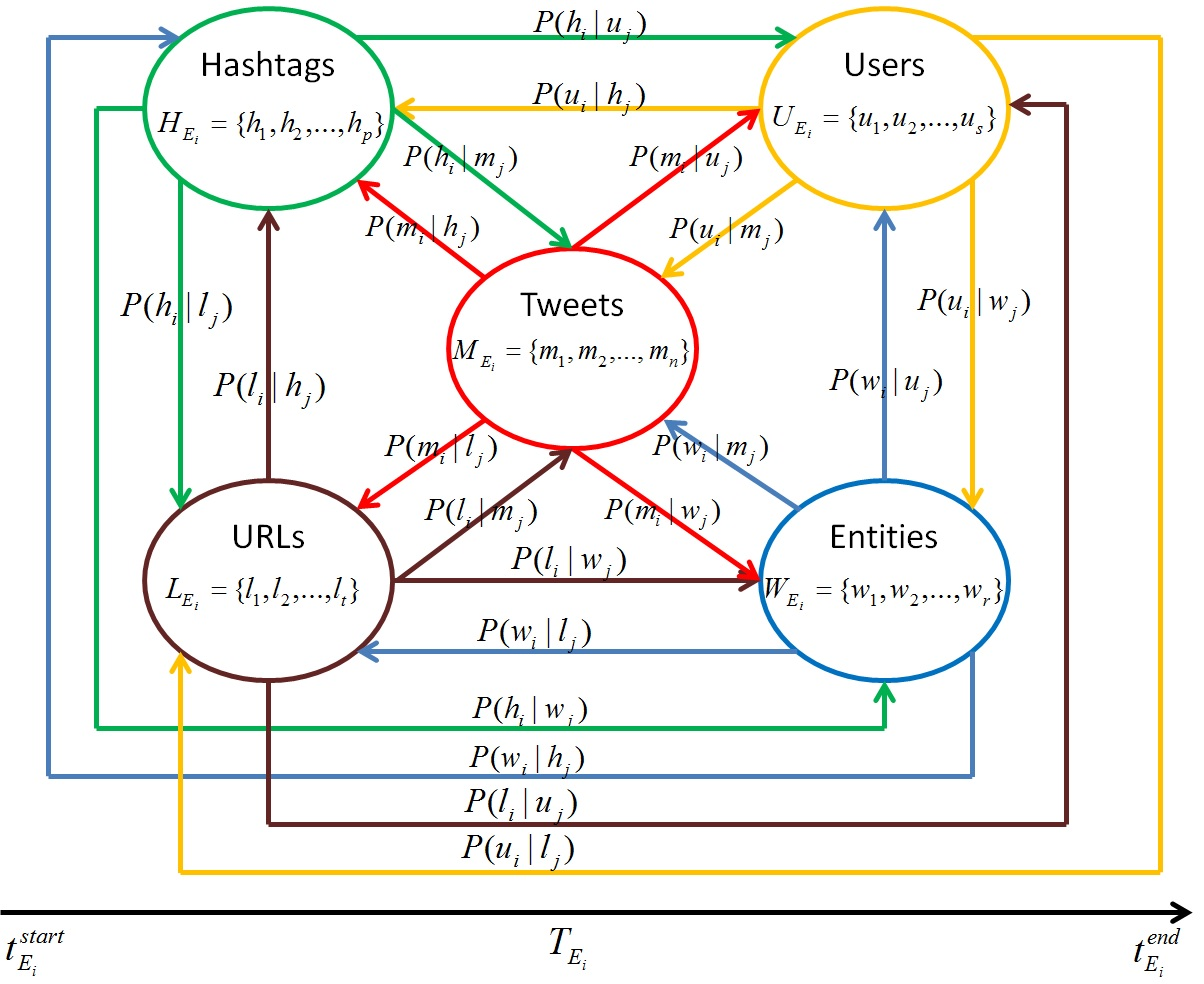
\includegraphics[width=16cm,height=12cm]{Figures/TwitterEventInfoGraph.jpg}
    
    \label{mrc}
\end{figure}

%\begin{table*}
%\caption{Conditional probabilities for calculating weights of the directed edges of graph G.}
%\label{edgescores}
%\begin{tabular}{|l|}
%\hline \\
%$\scriptstyle P(h_{i} \mid w_{j}) = \frac{No. \, of \, tweets \, h_{i} \, and \, w_{j} \, occur \, together}{No. \, of \, tweets \, w_{j} \, occurs}$, 
%$\scriptstyle P(w_{i} \mid h_{j}) = \frac{No. \, of \, tweets \, w_{i} \, and \, h_{j} \, occur \, together}{No. \, of \, tweets \, h_{j} \, occurs}$ , $\scriptstyle P(h_{i} \mid l_{j}) = \frac{No. \, of \, tweets \, h_{i} \, and \, l_{j} \, occur \, together}{No. \, of \, tweets \, l_{j} \, occurs}$,  \\
%
%$\scriptstyle P(l_{i} \mid h_{j}) = \frac{No. \, of \, tweets \, l_{i} \, and \, h_{j} \, occur \, together}{No. \, of \, tweets  \, h_{j} \, occurs}$, $\scriptstyle P(h_{i} \mid u_{j}) = \frac{No. \, of \, tweets  \, h_{i} \, and \, u_{j} \, occur \, together}{No. \, of \, tweets  \, u_{j} \, occurs}$ , $\scriptstyle P(u_{i} \mid h_{j}) = \frac{No. \, of \, tweets  \, u_{i} \, and \, h_{j} \, occur \, together}{No. \, of \, tweets  \, h_{j} \, occurs}$,  \\
%
%$\scriptstyle P(w_{i} \mid l_{j}) = \frac{No. \, of \, tweets  \, w_{i} \, and \, l_{j} \, occur \, together}{No. \, of \, tweets  \, l_{j} \, occurs}$, $\scriptstyle P(l_{i} \mid w_{j}) = \frac{No. \, of \, tweets  \, l_{i} \, and \, w_{j} \, occur \, together}{No. \, of \, tweets  \, w_{j} \, occurs}$, $\scriptstyle P(w_{i} \mid u_{j}) = \frac{No. \, of \, tweets  \, w_{i} \, and \, u_{j} \, occur \, together}{No. \, of \, tweets  \, u_{j} \, occurs}$, \\
%
%$\scriptstyle P(u_{i} \mid w_{j}) = \frac{No. \, of \, tweets  \, u_{i} \, and \, w_{j} \, occur \, together}{No. \, of \, tweets  \, w_{j} \, occurs}$, $\scriptstyle P(u_{i} \mid l_{j}) = \frac{No. \, of \, tweets  \, u_{i} \, and \, l_{j} \, occur \, together}{No. \, of \, tweets  \, l_{j} \, occurs}$, $\scriptstyle P(l_{i} \mid u_{j}) = \frac{No. \, of \, tweets  \, l_{i} \, and \, u_{j} \, occur \, together}{No. \, of \, tweets  \, u_{j} \, occurs}$, \\
%
%$\scriptstyle P(h_{i} \mid m_{j}) = P(m_{i} \mid h_{j}) = P(w_{i} \mid m_{j}) = P(m_{i} \mid w_{j}) = P(u_{i} \mid m_{j}) = P(m_{i} \mid u_{j}) = P(l_{i} \mid m_{j})= P(m_{i} \mid l_{j})= 1.0$ \\ 
%
%\scriptsize Note: $P(h_{i} \mid w_{j})$ should be read as the probability of occurrence of hashtag $h_{i}$ given the occurrence of the text unit $w_{j}$ in the stream of \scriptsize tweets $M_{E_{i}}$ related to event $E_{i}$ \\ \scriptsize collected over the time period $T_{E_{i}}. $\\
%\hline
%\end{tabular}
%
%\end{table*}

%\begin{itemize}
%\item 
For an event $E_{i}$ 
\begin{itemize} 
\item a \textit{tweet is an event-specific informative tweet} if it is strongly associated with:
\begin{itemize}
\item[\textbf{(a)}] \textit{event-specific informative hashtags}, 
\item[\textbf{(b)}] \textit{event-specific informative text units}, 
\item[\textbf{(c)}] \textit{event-specific informative users},
\item[\textbf{(d)}] \textit{event-specific informative URLs}. 
\end{itemize}
\end{itemize}

\begin{itemize} 
\item a \textit{hashtag is an event-specific informative hashtag} if it is strongly associated with:
\begin{itemize}
\item[\textbf{(a)}] \textit{event-specific informative tweets},
\item[\textbf{(b)}] \textit{event-specific informative text units},
\item[\textbf{(c)}] \textit{event-specific informative users},
\item[\textbf{(d)}] \textit{event-specific informative URLs}.
\end{itemize}
\end{itemize}

\begin{itemize} 
\item a \textit{text unit is an event-specific informative text unit} if it is strongly associated with:
\begin{itemize}
\item[\textbf{(a)}] \textit{event-specific informative tweets}, 
\item[\textbf{(b)}] \textit{event-specific informative hashtags}, 
\item[\textbf{(c)}] \textit{event-specific informative users}, 
\item[\textbf{(d)}] \textit{event-specific informative URLs}. 
\end{itemize}
\end{itemize}

\begin{itemize} 
\item a \textit{user is an event-specific informative user} if it is strongly associated with:
\begin{itemize}
\item[\textbf{(a)}] \textit{event-specific informative tweets}, 
\item[\textbf{(b)}] \textit{event-specific informative hashtags}, 
\item[\textbf{(c)}] \textit{event-specific informative text units},
\item[\textbf{(d)}] \textit{event-specific informative URLs}. 
\end{itemize}
\end{itemize}

\begin{itemize} \item a \textit{URL is an event-specific informative URL} if it is strongly associated with:
\begin{itemize}
\item[\textbf{(a)}] \textit{event-specific informative tweets}, 
\item[\textbf{(b)}] \textit{event-specific informative hashtags}, 
\item[\textbf{(c)}] \textit{event-specific informative text units},
\item[\textbf{(d)}] \textit{event-specific informative users}. 
\end{itemize}
\end{itemize}

%\end{itemize}

The relationships for an event $\scriptstyle E_{i}$ as stated above, forms a \textit{Mutual Reinforcement Chain} \cite{wei2008query} for the event $E_{i}$ as shown in Figure \ref{mrc}. We represent this relationship in a graph $\textbf{G = (V,D)}$, which we call as \textit{TwitterEventInfoGraph}, where $\mathbf{V = M_{E_{i}} \cup H_{E_{i}} \cup W_{E_{i}} \cup U_{E_{i}} \cup L_{E_{i}}}$, is the set of vertices and $\mathbf{D}$ is the set of directed edges between different vertices. 

Whenever two vertices are associated, there are two edges between them that are oppositely directed. Each directed edge is assigned a weight, which determines the degree of association of one vertex with the other. The weights for each edge is calculated according to the conditional probabilities given in Table \ref{edgescores}. 

We do not consider an edge between two vertices of same type. That is, we don't connect a tweet with another tweet. Similarly, for hashtags, text units, users and URLs. This constraint was imposed in order to deal with the nepotistic relationships between high quality content and low quality content introduced by the malicious users for promoting the low quality content. We observe these malicious side effects in the results obtained for \textit{TextRank} explained in Section 6.5.  

Next, we explain \textit{TwitterEventInfoRank}.

%%%%%%%%%%%%%%%%%%%%%%%%%%%%%%%%%%%%%%%%%%%%%%%%%%%%%%%%%%%%%%%%%%%%%%%%%%%%%%%%%%
%%%%%%%%%%%%%%%%%                                       TwitterEventInfoRank Subsection                    %%%%%%%%%%%%%%%%%%%%%%%%%%%%%%%%%%
%%%%%%%%%%%%%%%%%%%%%%%%%%%%%%%%%%%%%%%%%%%%%%%%%%%%%%%%%%%%%%%%%%%%%%%%%%%%%%%%%%

\subsection{TwitterEventInfoRank\label{twitterEventInfoRank}}
In this section, we introduce an iterative algorithm that takes into account the mutually reinforcing relationships between the vertices of \textit{TwitterEventInfoGraph} as explained in the previous section and propagates event-specific scores of each vertex to connected vertices across the graph for ranking its vertices ($\scriptstyle \in V$) in terms of event-specific informativeness.

We first assign a event-specific score to all the vertices of the graph. Event-specific scores for vertices $(\in H_{E_{i}}, W_{E_{i}}, U_{E_{i}}, L_{E_{i}})$ are calculated using equations (1-4) as presented in Table \ref{edgescores}. The tweets  $(\in M_{E_{i}})$ are assigned an initial informativeness score as obtained from the logistic regression model explained in Section 3. The event-specific scores for vertices $(\in H_{E_{i}}, W_{E_{i}}, U_{E_{i}}, L_{E_{i}})$ and informativeness score for vertices $(\in M_{E_{i}})$ gives an initial ranking of all the vertices of \textit{TwitterEventInfoGraph}. We aim to refine the initial scores and assign a final score for ranking the vertices by leveraging the mutually reinforcing relationships between them.
\begin{equation}
Score(h_{i}) = \frac{freq(h_{i})}{max\{freq(h_{1}),freq(h_{2}),...,freq(h_{p})\}}
\end{equation}

\begin{equation}
Score(w_{i}) = \frac{freq(w_{i})}{max\{freq(w_{1}),freq(w_{2}),...,freq(w_{r})\}}
\end{equation}

\begin{equation}
Score(u_{i}) = \frac{followers(u_{i})}{max\{followers(u_{1}),...,followers(u_{r})\}}
\end{equation}

\begin{equation}
Score(l_{i}) = \frac{freq(l_{i})}{max\{freq(l_{1}),freq(l_{2}),...,freq(l_{r})\}}
\end{equation}


The relationships between two different subsets of vertices in graph $\scriptstyle \mathbf{G}$ is denoted by an affinity matrix. For e.g., $\mathbf{A_{E_{i}}^{MH}}$ denotes the $\mathbf{M_{E_{i}}-H_{E_{i}}}$ affinity matrix for event $E_{i}$, where $\mathbf{(i,j)^{th}}$ entry is the edge weight quantifying the association between $i^{th}$ tweet ($\in M_{E_{i}}$) and $j^{th}$ hashtag ($\in H_{E_{i}}$), calculated using Table \ref{edgescores}. Similarly, $\mathbf{A_{E_{i}}^{WH}}$ denotes the $\mathbf{W_{E_{i}}-H_{E_{i}}}$ affinity matrix between set of text units $W_{E_{i}}$ and set of hashtags $H_{E_{i}}$ for event $E_{i}$, and so on.


The rankings of \textit{tweets}, \textit{hashtags}, \textit{text units}, \textit{users} and \textit{URLs} in terms of event-specific informativeness, can be iteratively derived from the Mutual Reinforcement Chain for the event. Let $R_{{E_{i}}}^{M}$, $R_{{E_{i}}}^{H}$, $R_{{E_{i}}}^{W}$, $R_{{E_{i}}}^{U}$ and $\scriptstyle R_{{E_{i}}}^{L}$ denote the ranking scores for the set of tweets ($\in M_{E_{}}$), set of  hashtags $(\in H_{E_{i}})$, set of text units $(\in W_{E_{i}})$, set of users $(\in U_{E_{i}})$, and set of URLs $(\in L_{E_{i}})$, respectively. Therefore, the Mutual Reinforcement Chain ranking for the $k^{th}$ iteration can be formulated as follows:
 

%\begin{equation}
%\tiny R_{{E_{i}}}^{M(k+1)} = A_{E_{i}}^{MM(k)}R_{{E_{i}}}^{M(k)} + A_{E_{i}}^{MH(k)}R_{{E_{i}}}^{H(k)} + A_{E_{i}}^{MW(k)}R_{{E_{i}}}^{W(k)} + A_{E_{i}}^{MU(k)}R_{{E_{i}}}^{U(k)} + A_{E_{i}}^{ML(k)}R_{{E_{i}}}^{L(k)}
%\end{equation}

\begin{equation}
R_{{E_{i}}}^{M(k+1)} = A_{E_{i}}^{MM(k)}R_{{E_{i}}}^{M(k)} + A_{E_{i}}^{MH(k)}R_{{E_{i}}}^{H(k)} + A_{E_{i}}^{MW(k)}R_{{E_{i}}}^{W(k)}+ A_{E_{i}}^{MU(k)}R_{{E_{i}}}^{U(k)} + A_{E_{i}}^{ML(k)}R_{{E_{i}}}^{L(k)}
\end{equation}

%\begin{equation}
%\tiny R_{{E_{i}}}^{H(k+1)} = A_{E_{i}}^{HM(k)}R_{{E_{i}}}^{M(k)} + A_{E_{i}}^{HH(k)}R_{{E_{i}}}^{H(k)} + A_{E_{i}}^{HW(k)}R_{{E_{i}}}^{W(k)} + A_{E_{i}}^{HU(k)}R_{{E_{i}}}^{U(k)} + A_{E_{i}}^{HL(k)}R_{{E_{i}}}^{L(k)}
%\end{equation}

\begin{equation}
R_{{E_{i}}}^{H(k+1)} = A_{E_{i}}^{HM(k)}R_{{E_{i}}}^{M(k)} + A_{E_{i}}^{HH(k)}R_{{E_{i}}}^{H(k)} + A_{E_{i}}^{HW(k)}R_{{E_{i}}}^{W(k)}+ A_{E_{i}}^{HU(k)}R_{{E_{i}}}^{U(k)} + A_{E_{i}}^{HL(k)}R_{{E_{i}}}^{L(k)}
\end{equation}



%\begin{equation}
%\tiny R_{{E_{i}}}^{W(k+1)} = A_{E_{i}}^{WM(k)}R_{{E_{i}}}^{M(k)} + A_{E_{i}}^{WH(k)}R_{{E_{i}}}^{H(k)} + A_{E_{i}}^{WW(k)}R_{{E_{i}}}^{W(k)} + A_{E_{i}}^{WU(k)}R_{{E_{i}}}^{U(k)} + A_{E_{i}}^{WL(k)}R_{{E_{i}}}^{L(k)}
%\end{equation}

\begin{equation}
R_{{E_{i}}}^{W(k+1)} = A_{E_{i}}^{WM(k)}R_{{E_{i}}}^{M(k)} + A_{E_{i}}^{WH(k)}R_{{E_{i}}}^{H(k)} + A_{E_{i}}^{WW(k)}R_{{E_{i}}}^{W(k)}+ A_{E_{i}}^{WU(k)}R_{{E_{i}}}^{U(k)} + A_{E_{i}}^{WL(k)}R_{{E_{i}}}^{L(k)}
\end{equation}

%\begin{equation}
%\tiny R_{{E_{i}}}^{U(k+1)} = A_{E_{i}}^{UM(k)}R_{{E_{i}}}^{M(k)} + A_{E_{i}}^{UH(k)}R_{{E_{i}}}^{H(k)} + A_{E_{i}}^{UW(k)}R_{{E_{i}}}^{W(k)} + A_{E_{i}}^{UU(k)}R_{{E_{i}}}^{U(k)} + A_{E_{i}}^{UL(k)}R_{{E_{i}}}^{L(k)}
%\end{equation}

\begin{equation}
R_{{E_{i}}}^{U(k+1)} = A_{E_{i}}^{UM(k)}R_{{E_{i}}}^{M(k)} + A_{E_{i}}^{UH(k)}R_{{E_{i}}}^{H(k)} + A_{E_{i}}^{UW(k)}R_{{E_{i}}}^{W(k)}+ A_{E_{i}}^{UU(k)}R_{{E_{i}}}^{U(k)} + A_{E_{i}}^{UL(k)}R_{{E_{i}}}^{L(k)}
\end{equation}

%\begin{equation}
%\tiny R_{{E_{i}}}^{L(k+1)} = A_{E_{i}}^{LM(k)}R_{{E_{i}}}^{M(k)} + A_{E_{i}}^{LH(k)}R_{{E_{i}}}^{H(k)} + A_{E_{i}}^{LW(k)}R_{{E_{i}}}^{W(k)} + A_{E_{i}}^{LU(k)}R_{{E_{i}}}^{U(k)} + A_{E_{i}}^{LL(k)}R_{{E_{i}}}^{L(k)}
%\end{equation}


\begin{equation}
R_{{E_{i}}}^{L(k+1)} = A_{E_{i}}^{LM(k)}R_{{E_{i}}}^{M(k)} + A_{E_{i}}^{LH(k)}R_{{E_{i}}}^{H(k)} +A_{E_{i}}^{LW(k)}R_{{E_{i}}}^{W(k)}+ A_{E_{i}}^{LU(k)}R_{{E_{i}}}^{U(k)}+ A_{E_{i}}^{LL(k)}R_{{E_{i}}}^{L(k)}
\end{equation}


The equations 5-9 can be represented in the form of a block matrix $\Delta_{E_{i}}$, where,
\[ \Delta_{E_{i}} = \left( \begin{array}{ccccc}
A_{E_{i}}^{MM} & A_{E_{i}}^{MH} & A_{E_{i}}^{MW} &  A_{E_{i}}^{MU} & A_{E_{i}}^{ML} \\
A_{E_{i}}^{HM} & A_{E_{i}}^{HH} & A_{E_{i}}^{HW} & A_{E_{i}}^{HU} & A_{E_{i}}^{HL} \\
A_{E_{i}}^{WM} & A_{E_{i}}^{WH} & A_{E_{i}}^{WW} & A_{E_{i}}^{WU} & A_{E_{i}}^{WL}\\
A_{E_{i}}^{UM} & A_{E_{i}}^{UH} & A_{E_{i}}^{UW} & A_{E_{i}}^{UU} & A_{E_{i}}^{UL} \\
A_{E_{i}}^{LM} & A_{E_{i}}^{LH} & A_{E_{i}}^{LW} & A_{E_{i}}^{LU} & A_{E_{i}}^{LL} \end{array} \right)\] 

Let \[R_{E_{i}} = \left( \begin{array}{c}
R_{{E_{i}}}^{M} \\
R_{{E_{i}}}^{H} \\
R_{{E_{i}}}^{W} \\
R_{{E_{i}}}^{U} \\
R_{{E_{i}}}^{L} \end{array} \right)\] 

then, $R_{E_{i}}$ can be computed as the dominant eigenvector of $\Delta_{E_{i}}$.
\begin{equation}
\Delta_{E_{i}}.R_{E_{i}} = \lambda.R_{E_{i}}
\end{equation}

In order to guarantee a unique $R_{E_{i}}$, $\Delta_{E_{i}}$ must be forced to be stochastic and irreducible. 

To make $\Delta_{E_{i}}$ stochastic we divide the value of each element in a column of $\Delta_{E_{i}}$ by the sum of the values of all the elements in that column. This finally makes $\Delta_{E_{i}}$ column stochastic. We now denote it by $\hat \Delta_{E_{i}}$.
%we remove all the rows and columns of the block matrices whose all elements are zeros. Since, we don't consider edges between two vertices of same type, all the elements of the diagonal block matrices are zero by default. We then 

Next, we make $\hat \Delta_{E_{i}}$ irreducible. This is done by making the graph $G$ strongly connected by adding links from one node to any other node with a probability vector $p$. Now, $\hat \Delta_{E_{i}}$ is transformed to 

\begin{equation}
\overline \Delta_{E_{i}} = \alpha \hat \Delta_{E_{i}} + (1-\alpha)E
\end{equation}
\begin{equation}
E = p \times [1]_{1 \times k}
\end{equation}
where $0 \le \alpha \le 1$ is set to 0.85 according to \textit{PageRank}, and k is the order of $\hat \Delta_{E_{i}}$. We set $p = [1/k]_{k \times 1}$ by assuming a uniform distribution over all elements. Now, $\overline \Delta_{E_{i}}$ is stochastic and irreducible and it can be shown that it is also primitive by checking $\overline \Delta_{E_{i}}^{2}$ is greater than $0$.

Following steps are taken next,
\begin{itemize}
\item[\textbf{1.}] We initialize the rank vectors ($ R_{{E_{i}}}^{M(0)}, R_{{E_{i}}}^{H(0)}, R_{{E_{i}}}^{W(0)}, R_{{E_{i}}}^{U(0)}, R_{{E_{i}}}^{L(0)}$) for each subset of vertices ($M_{E_{i}}, H_{E_{i}}, W_{E_{i}}, U_{E_{i}}, L_{E_{i}}$). We use the event-specific scores calculated for the set of hashtags, text units, users and urls as their initial scores. All the scores lie between 0 and 1. For the tweets we use the logistic regression model and assign each one of them an initial informativeness score between 0 and 1.

\item[\textbf{2.}] Then we assign
\[ R_{E_{i}}^{0} = \left( \begin{array}{c}
R_{{E_{i}}}^{M(0)} \\
R_{{E_{i}}}^{H(0)} \\
R_{{E_{i}}}^{W(0)} \\
R_{{E_{i}}}^{U(0)} \\
R_{{E_{i}}}^{L(0)} \end{array} \right)\] 

and normalize $R_{E_{i}}^{0}$ such that $\mid \mid R_{E_{i}}^{0}\mid \mid_{1} = 1$

\item[\textbf{3.}] Apply power iteration method using the same parameters as used in PageRank with the convergence tolerance set at 1e-08 and $\lambda = 0.85$ .

\item[\textbf{4.}] We get the final rank vectors for each subset of the vertices ($R_{{E_{i}}}^{M}, R_{{E_{i}}}^{H}, R_{{E_{i}}}^{W}, R_{{E_{i}}}^{U}, R_{{E_{i}}}^{L}$) after convergence. 

\item[\textbf{5.}] We finally obtain the subsets $\hat{M}_{E_{i}}, \hat{H}_{E_{i}}, \hat{W}_{E_{i}}, \hat{L}_{E_{i}}, \hat{U}_{E_{i}}$ consisting of the \textit{tweets}, \textit{hashtags}, \textit{text units}, \textit{URLs} and \textit{users}, respectively arranged in descending order of their final scores.

\end{itemize}

The final ordered subsets $\scriptstyle \mathbf{\hat{M}_{E_{i}}, \hat{H}_{E_{i}}, \hat{W}_{E_{i}}, \hat{L}_{E_{i}}, \hat{U}_{E_{i}}}$,  thus obtained are the tweets, hashtags, text units, URLs and users, ranked in terms of their event-specific informativeness. 

\begin{algorithm}
\label{algo}
\SetKwData{Left}{left}\SetKwData{This}{this}\SetKwData{Up}{up}
\SetKwFunction{Union}{Union}\SetKwFunction{FindCompress}{FindCompress}
\SetKwInOut{Input}{Input}\SetKwInOut{Output}{Output}
\Input{Sets of vertices $M_{E_{i}},H_{E_{i}}, W_{E_{i}}, U_{E_{i}}, L_{E_{i}}$ of graph G, $\alpha=0.85$, $\varepsilon=1e-08$.}
\BlankLine
\Output{Ordered set of vertices $\hat{M}_{E_{i}}$, containing tweets ranked in order of event-specific informative content sharing information about event related entities.}
\BlankLine
\textbf{Steps:}
\BlankLine
Initialize rank vectors $[R_{{E_{i}}}^{M(0)}, R_{{E_{i}}}^{H(0)}, R_{{E_{i}}}^{W(0)}, R_{{E_{i}}}^{U(0)}, R_{{E_{i}}}^{L(0)}]$\;
\BlankLine
Assign $R_{E_{i}}^{0}=[R_{E_{i}}^{M(0)},R_{E_{i}}^{H(0)},R_{E_{i}}^{W(0)},R_{E_{i}}^{U(0)},R_{E_{i}}^{L(0)}]^{T} $\;
\BlankLine
Normalize $R_{E_{i}}^{0}$ such that $\mid \mid R_{E_{i}}^{0}\mid \mid_{1} = 1$ \;
\BlankLine
Construct matrix $\Delta_{E_{i}}$\;
\BlankLine
Make matrix $\Delta_{E_{i}}$ stochastic and irreducible converting it to $\overline \Delta_{E_{i}}$\;
\BlankLine
$k \leftarrow 1$ 
\BlankLine
\Repeat{$\mid \mid R_{E_{i}}^{k} - R_{E_{i}}^{k-1} \mid \mid_{1} < \varepsilon \; OR \; k \ge 100$}{$R_{E_{i}}^{k} \leftarrow \overline \Delta_{E_{i}}R_{E_{i}}^{k-1}$\;
$k \leftarrow k+1$\; }
\BlankLine
$R_{E_{i}}^{M} \leftarrow R_{E_{i}}^{M(k)}$, $R_{E_{i}}^{H} \leftarrow R_{E_{i}}^{H(k)}$, $R_{E_{i}}^{W} \leftarrow R_{E_{i}}^{W(k)}$,  $R_{E_{i}}^{U} \leftarrow R_{E_{i}}^{U(k)}$, $R_{E_{i}}^{L} \leftarrow R_{E_{i}}^{L(k)}$\;
\BlankLine
$\hat{M}_{E_{i}} \leftarrow R_{E_{i}}^{M}$, $\hat{H}_{E_{i}} \leftarrow R_{E_{i}}^{H}$, $\hat{W}_{E_{i}} \leftarrow R_{E_{i}}^{W}$, $\hat{U}_{E_{i}} \leftarrow R_{E_{i}}^{U}$, $\hat{L}_{E_{i}} \leftarrow R_{E_{i}}^{L}$\;
\BlankLine
return $\hat{M}_{E_{i}}$,$\hat{H}_{E_{i}}$,$\hat{W}_{E_{i}}$,$\hat{U}_{E_{i}}$,$\hat{L}_{E_{i}}$\;
%\caption{\scriptsize Algorithm for ranking the nodes of G}\label{algo_disjdecomp}
\end{algorithm}\DecMargin{1em}

During the implementation of the \textit{TwitterEventInfoRank} algorithm the slang hashtags were removed. We only considered nouns as the text units and removed the slang words. We already reported in our analysis that non-informative tweets have higher slang content. Therefore, removal of slang hashtags and text units was done in order to obtain high quality results. We also showed higher occurrence of nouns in informative tweets. Also, the occurrence of a noun in a tweet intuitively suggests that the tweet has information about a person, place, or thing. Thus, we only considered the set of nouns extracted from the tweets as the set of text units. 

The text units are generic units in the framework and can be changed according to specific requirements. Entities extracted from the textual content of tweets could be experimented, in place of nouns. Since the algorithm uses power iteration method for ranking the vertices of the graph, it could be easily made scalable using mapreduce paradigm \cite{lin2010design}. We plan to work on it in the future and implement our framework using hadoop and mapreduce environment. 

Since, our proposed framework takes a hybrid approach by using both supervised and unsupervised component, it is easily applicable in situations where an event needs to be tracked over time. The supervised portion assigns an initial generic informativeness score to the tweets for bootstrapping an unsupervised process that finally assigns event-specific informativeness scores. When applied over a time period the method for assigning the initial supervised scores might remain the same and the unsupervised process can change the rankings of the tweet contents as the event evolves. 

Next, we present details of experimental settings and evaluation.
  
%%%%%%%%%%%%%%%%%%%%%%%%%%%%%%%%%%%%%%%%%%%%%%%%%%%%%%%%%%%%%%%%%%%%%%%%%%%%%%%%%%
%%%%%%%%%%%%%%%%%                                       Experiments Section                    %%%%%%%%%%%%%%%%%%%%%%%%%%%%%%%%%%%%%%%%
%%%%%%%%%%%%%%%%%%%%%%%%%%%%%%%%%%%%%%%%%%%%%%%%%%%%%%%%%%%%%%%%%%%%%%%%%%%%%%%%%%

%\section{Experiments}

%%%%%%%%%%%%%%%%%%%%%%%%%%%%%%%%%%%%%%%%%%%%%%%%%%%%%%%%%%%%%%%%%%%%%%%%%%%%%%%%%%
%%%%%%%%%%%%%%%%%                           Experimental Settings Subsection                    %%%%%%%%%%%%%%%%%%%%%%%%%%%%%%%%%%%%%
%%%%%%%%%%%%%%%%%%%%%%%%%%%%%%%%%%%%%%%%%%%%%%%%%%%%%%%%%%%%%%%%%%%%%%%%%%%%%%%%%%

\section{Experimental Settings and Evaluation\label{experimentalSettingsAndEvaluation}}
In this section, we explain the settings of the experiment conducted by us. We give the details of the data collected for performing the experiment. All the data preparation steps used for preprocessing the tweets before analyzing them and applying the algorithms are explained. We present the baselines used for comparing the effectiveness of our proposed algorithm and perform the evaluation tasks. We go through the evaluation results and discuss about the performance of our algorithm. 

Next, we present details of the data collected for the experiment.

\subsection{Data Collection\label{dataCollection}}


\begin{table}
\center
\caption{Details of data collected for the experiment.}
\label{experimentdata}
\begin{tabular}{|c|c|c|}
\hline
\shortstack{\textbf{Event Name}\\ \textbf{and Query Hashtag}}                            & \shortstack{\textbf{No. of} \\ \textbf{Tweets}} & \shortstack{\textbf{Time Period} \\ \textbf{(UTC)}}                               \\ \hline
\shortstack{Millions March \\ NYC\\ (\#millionsmarchnyc) \\ ($http://goo.gl/I8WR4B$)} & 56927 & \shortstack{13th Dec, 2014\\ 20:25:43\\ to\\ 14th Dec, 2014\\ 03:30:41} \\ \hline
%\begin{tabular}[c]{@{}c@{}}Millions March \\ NYC\\ (\#millionsmarchnyc)\end{tabular}                    & 56927                                                             & \begin{tabular}[c]{@{}c@{}}13th Dec, 2014\\ 20:25:43\\ to\\ 14th Dec, 2014\\ 03:30:41\end{tabular} \\ \hline
\begin{tabular}[c]{@{}c@{}}Sydney Siege\\ (\#sydneysiege) \\ ($http://goo.gl/qLguvG$)\end{tabular}                                  & 398204                                                            & \begin{tabular}[c]{@{}c@{}}15th Dec, 2014\\ 07:21:16\\ to\\ 15th Dec, 2014\\ 22:46:45\end{tabular} \\ \hline
%\begin{tabular}[c]{@{}c@{}}Heats Vs\\ Cavaliers\\ Xmas Game\\ (\#heatvscavs) \\ ($http://goo.gl/9G5NxW$)\end{tabular} & 2947                                                              & \begin{tabular}[c]{@{}c@{}}25th Dec, 2014\\ 20:45:29\\ to\\ 26th Dec, 2014\\ 16:13:46\end{tabular} \\ \hline
\end{tabular}
\end{table}


For implementing and evaluating our proposed algorithm we collected 455,131 tweets from two real-life events, `Millions March NYC' and `Sydney Siege', using Twitter Streaming API. Details of the dataset is presented in Table \ref{experimentdata}.
Tweets for each event was collected over the given period of time, by providing a popular hashtag corresponding to each event to the Twitter streaming API. The events for the experiments are different from the events selected for initial analysis as the choice was driven by its availability in Seen.co event database, whose ranking scores\footnote{\tiny Tweets in Seen.co is ranked according to their proprietary algorithm SeenRank and the scores are available in the response of their API found at (http://developer.seen.co/) We used a python wrapper freely available at https://github.com/dxmahata/pySeen for collecting data from Seen.co} are used as one of the baselines representing the state-of-the-art technique.

%by its different nature (Protest, Terrorism and Sports) and its coverage by
%Seen.co \footnote{http://seen.co/about}, whose ranking scores\footnote{\tiny Tweets in Seen.co is ranked according to their proprietary algorithm SeenRank and the scores are available in the response of their API found at (http://developer.seen.co/). We used a python wrapper freely available at https://github.com/dxmahata/pySeen for collecting data from Seen.co} are used as one of the baselines representing the state-of-the-art technique.



\subsection{Data Preparation\label{dataprep}}
We performed a series of data preparation steps before analyzing the tweets and implementing the \textit{TwitterEventInfoRank} algorithm.  Tweets having duplicate content were detected using md5 hashing scheme, and redundant copies were filtered out keeping a single representation of the tweet in our database. Although, the methodology is language independent,
we only considered English language tweets, as the manual annotators used for evaluation were only proficient in English. Also the natural language toolkits used for the work gave best results for English text. 

We used the default parts-of-speech (POS) tagging module provided by NLTK library\footnote{\tiny http://nltk.org}. A standard list of english stop words was used for eliminating the stop words from tweet text. All the characters of the tweets were converted to lower case. The tweets were tokenized after detecting the POS tags and removing the special characters. We filtered out the user mentions, retweet symbol (\textit{RT}) and URLs from the text during tokenization and did not consider them as tokens. A list of words expressing feelings was obtained from \textit{wefeelfine.org}. Twitter related slang words were obtained from a publicly available document published by United States FBI\footnote{\tiny https://www.documentcloud.org/documents/1199460-responsive-documents.html\#document/p1}. A final list of slang words was compiled 
by adding some more internet slangs. The list would be made available on request. Retweet counts, favorite counts, verification information, user followers count and time information were obtained from the metadata attached with each tweet returned by Twitter API. The URLs shared in tweets are generally shortened. Due to the use of different URL shortener services, a single URL might be represented in different forms by each service. In order to solve this problem, we used AlchemyAPI\footnote{\tiny http://alchemyapi.com} to expand the URLs to their original form.

%Also, we considered only nouns based on our intuition that the tweets containing nouns have higher chances of providing information and present content about some person, place, or thing.



\subsection{Experiment with Named Entities as Text Units}
\subsubsection{Baselines}
\subsection{Experiment with Nouns as Text Units}
\subsubsection{Baselines}
In order to evaluate the performance of \textit{TwitterEventInfoRank} we selected six different algorithms that acted as our baselines. Please refer to the \textit{Related Work} section (Section 2) for pointers to scientific literature explaining the techniques. Three of the baseline algorithms \textit{LexRank}, \textit{TextRank}, \textit{Centroid} are widely used by the scientific community. Among the other three, one of them is a proprietary algorithm known as \textit{SeenRank} commercially used by Seen.co for generating event summaries and highlights from Twitter. We considered \textit{SeenRank} as the state-of-the-art technique. The other one is the Logistic Regression model that we implemented for initializing the informativeness score of the tweets. We considered it in order to make sure that our algorithm improves upon the initial generic informativeness score already assigned to the tweets at the start of the iteration and assigns event-specific informativeness scores on convergence. Number of retweets is a good measure of popularity of a tweet and is also used by Twitter for ranking its search results. Therefore, we also considered tweets ordered in decreasing order of number of retweets as one of our baselines. We name this scheme as \textit{RTRank}

\textit{Centroid} is one of the techniques that was previously used in the literature for solving a part of our problem that ranks tweets. In order to implement it as a baseline we considered the tweets for the event in the given time period as one cluster. After preprocessing the tweets, we calculated the centroid of the cluster and ordered the tweets in the decreasing order of their similarities with the centroid. We selected \textit{LexRank} and \textit{TextRank}, as they are graph-based techniques for ranking textual documents, and are widely used for generating summaries.  We used the open-source implementation of \textit{LexRank} available with sumy\footnote{\tiny https://pypi.python.org/pypi/sumy/0.1.0} package. In case of \textit{TextRank}, we modified the algorithm in order to make it suitable for our context. Apart from creating heterogeneous relationships in \textit{TwitterEventInfoGraph} we also created homogeneous relationships between the \textit{information units} as well as the tweets. Cosine similarity ($ \ge 0.10$) was used as the measure of relatedness between tweets, and the association scores of the hashtags, text units, users and URLs were based on their co-occurrence normalized between 0 and 1. The users were associated whenever they mentioned each other in the tweets, and the association score was measured by the number of mentions normalized between 0 and 1.
%Number of retweets is used by Twitter for ranking its search results and is also a good indicator of popularity of a tweet. We decided to consider tweets ordered in decreasing order of number of retweets as one of our baselines. Since our algorithm has similarities with graph-based summarization techniques we selected two graph-based summarization algorithms, \textit{LexRank} and \textit{TextRank} as baselines as well.

Due to unavailability of proper baseline techniques for ranking hashtags, text units, URLs and users in terms of event-specific informativeness we do not compare the results obtained for them with any other approach. However, we report their average scores and sample results.

\begin{figure}[htbp]
\centering
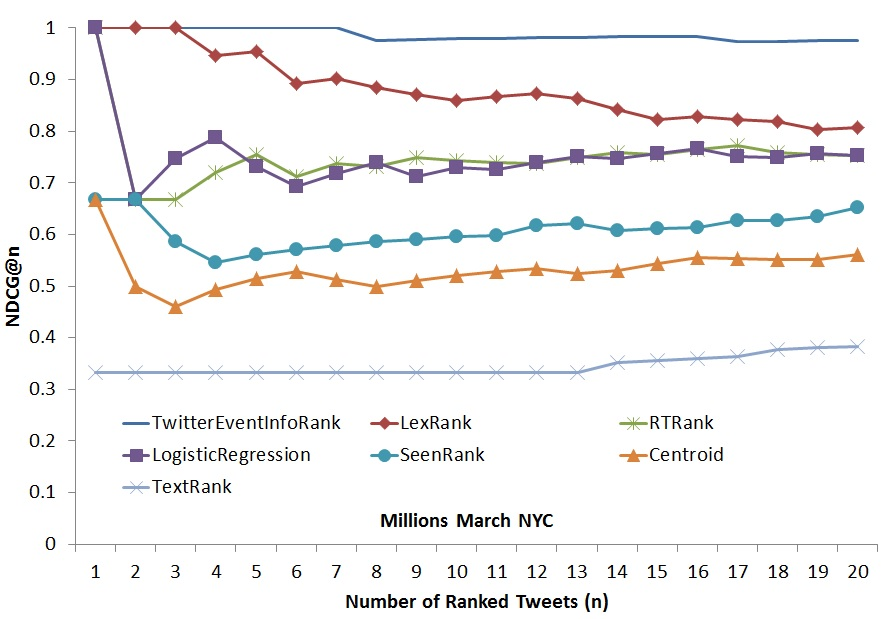
\includegraphics[height=4.5in,width=6in]{Figures/Chapter4Figures/MillionsMarchNycEventIdentityInfoRankPerformance.jpg}
\caption{\small Performance comparison of ranking techniques using NDCG scores.}
\label{millionsmarchndcg}
\end{figure}

\begin{figure}[htbp]
\centering
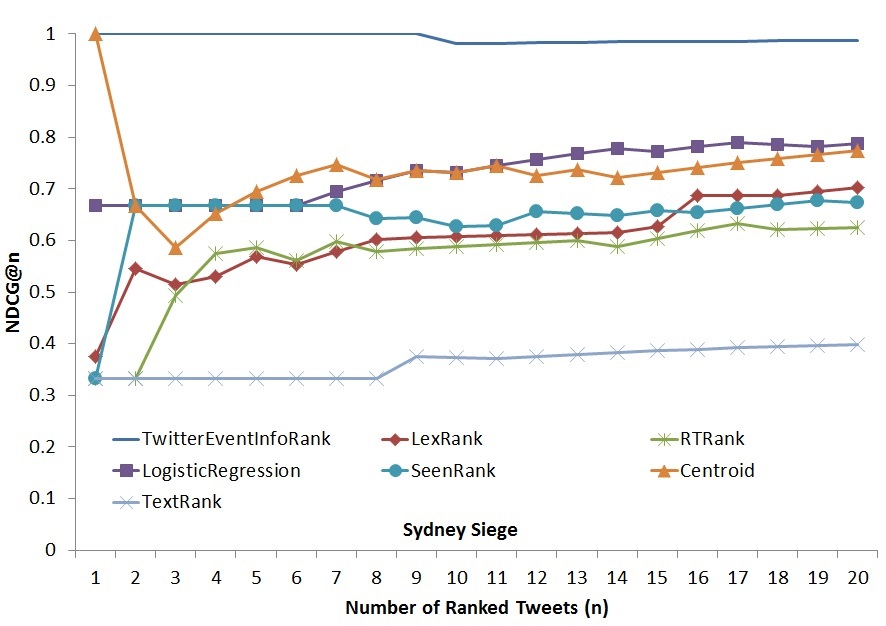
\includegraphics[height=4.5in,width=6in]{Figures/Chapter4Figures/SydneySiegeEventIdentityInfoRankPerformance.jpg}
\caption{\small Performance comparison of ranking techniques using NDCG scores.}
\label{sydneysiegendcg}
\end{figure}


\begin{table}[htbp]
\centering
\caption{Avg IIC scores and total avg scores of annotations for Millions March NYC event.}
\label{avgiicMillionsMarchNyc}
\begin{tabular}{|c|c|c|}
\hline
\textbf{\begin{tabular}[c]{@{}c@{}}Millions March \\ NYC\end{tabular}} & \textbf{IIC} & \textbf{\begin{tabular}[c]{@{}c@{}}Total Avg \\ Score (1-3)\end{tabular}} \\ \hline
\textbf{\begin{tabular}[c]{@{}c@{}}Top 50 event-specific\\ informative Hashtags\end{tabular}} & 0.786 & 1.980 \\ \hline
\textbf{\begin{tabular}[c]{@{}c@{}}Top 50 event-specific\\ informative Text Units\end{tabular}} & 0.880 & 1.320 \\ \hline
\textbf{\begin{tabular}[c]{@{}c@{}}Top 50 event-specific\\ informative URLs\end{tabular}} & 0.926 & 2.560 \\ \hline
\textbf{\begin{tabular}[c]{@{}c@{}}Top 50 event-specific\\ informative Users\end{tabular}} & 0.700 & 2.386 \\ \hline
\textbf{\begin{tabular}[c]{@{}c@{}}Top 100 event-specific\\ informative Tweets\end{tabular}} & 0.760 & 2.59 \\ \hline
\end{tabular}
\end{table}



\begin{table}[htbp]
\centering
\caption{Avg IIC scores and total avg scores of annotations for Sydney Siege event.}
\label{avgiicSydneySiege}
\begin{tabular}{|c|c|c|}
\hline
\textbf{Sydney Siege} & \textbf{IIC} & \textbf{\begin{tabular}[c]{@{}c@{}}Total Avg\\ Score (1-3)\end{tabular}} \\ \hline
\textbf{\begin{tabular}[c]{@{}c@{}}Top 50 event-specific\\ informative Hashtags\end{tabular}} & 0.880 & 2.027 \\ \hline
\textbf{\begin{tabular}[c]{@{}c@{}}Top 50 event-specific\\ informative Text Units\end{tabular}} & 0.986 & 1.487 \\ \hline
\textbf{\begin{tabular}[c]{@{}c@{}}Top 50 event-specific\\ informative URLs\end{tabular}} & 0.893 & 2.413 \\ \hline
\textbf{\begin{tabular}[c]{@{}c@{}}Top 50 event-specific\\ informative Users\end{tabular}} & 0.646 & 2.353 \\ \hline
\textbf{\begin{tabular}[c]{@{}c@{}}Top 100 event-specific\\ informative Tweets\end{tabular}} & 0.83 & 2.62 \\ \hline
\end{tabular}
\end{table}

\begin{figure}[htbp]
\centering
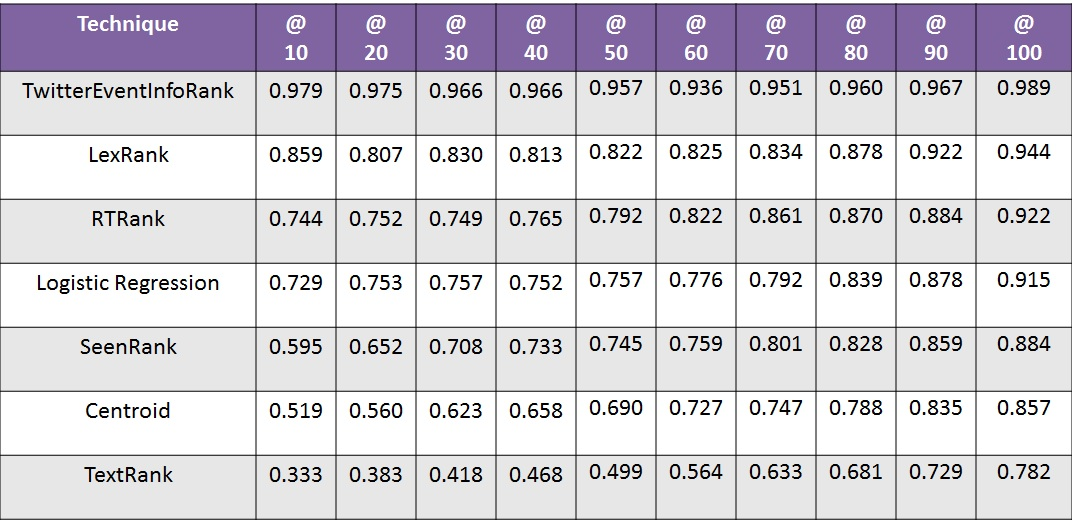
\includegraphics[height=3.5in,width=5.5in]{Figures/millionsmarchnycndcg.jpg}
\caption{\small Performance comparison of ranking techniques using NDCG scores.}
\label{millionsmarchndcg}
\end{figure}

\begin{figure}[htbp]
\centering
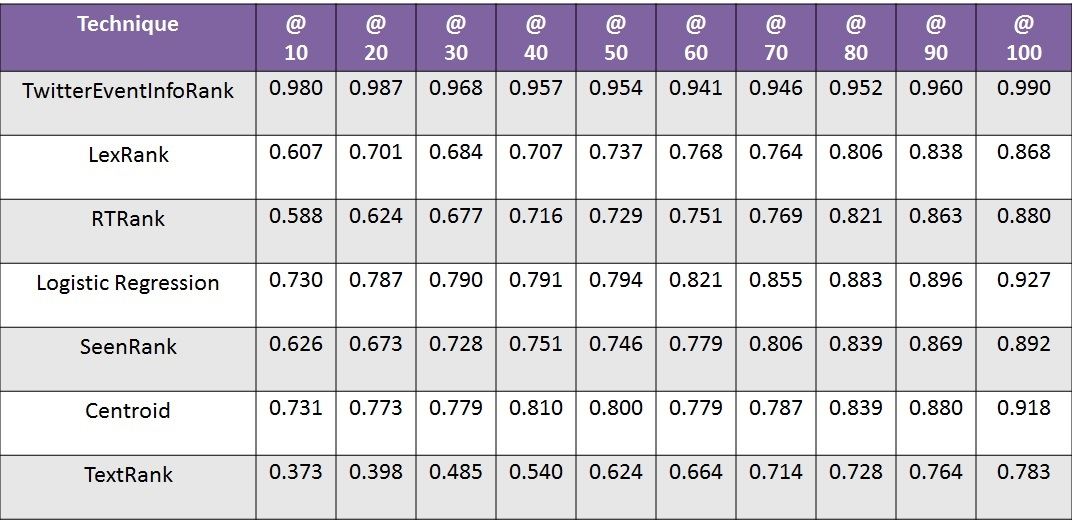
\includegraphics[height=3.5in,width=5.5in]{Figures/sydneysiegendcg.jpg}
\caption{\small Performance comparison of ranking techniques using NDCG scores.}
\label{sydneysiegendcg}
\end{figure}

\begin{figure}[htbp]
\centering
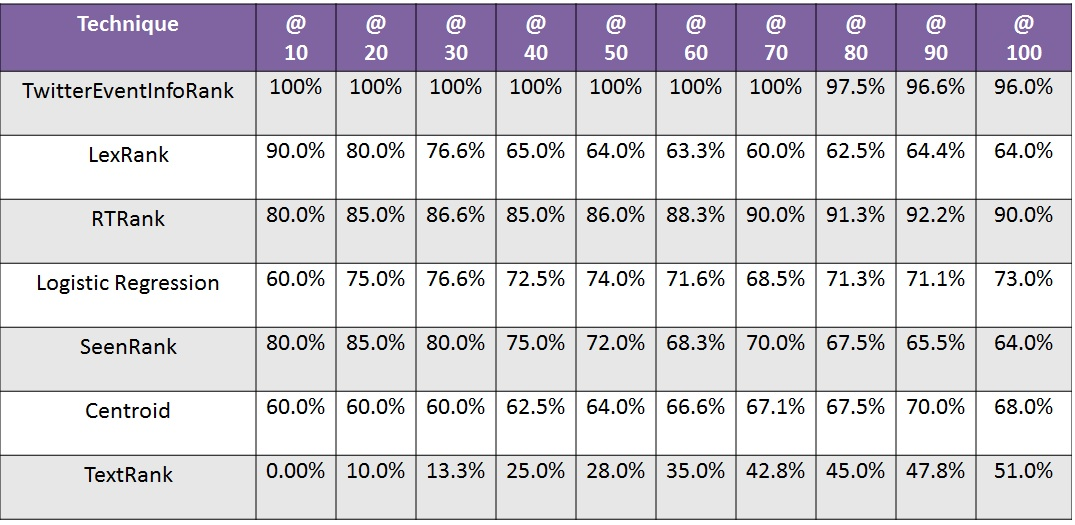
\includegraphics[height=3.5in,width=5.5in]{Figures/millionsmarchnycprecision.jpg}
\caption{\small Performance comparison of ranking techniques using precision scores.}
\label{millionsmarchnycprecision}
\end{figure}

\begin{figure}[htbp]
\centering
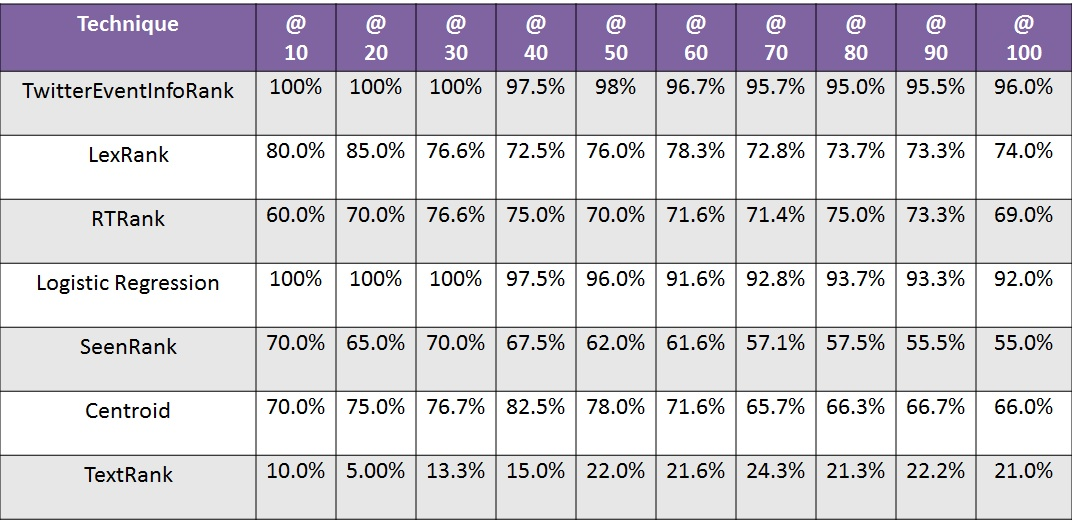
\includegraphics[height=3.5in,width=5.5in]{Figures/sydneysiegeprecision.jpg}
\caption{\small Performance comparison of ranking techniques using precision scores.}
\label{sydneysiegeprecision}
\end{figure}


%\begin{table}[ht]
%\tiny
%\centering
%\caption{\small NDCG@n and Precision@n scores for different techniques applied for ranking tweets related to Millions March NYC.}
%\label{millionpre}
%\begin{tabular}{|cc|c|c|c|c|c|c|c|c|c|c|}
%\cline{1-12}
%\textbf{Event Name: Millions March NYC}& & \multicolumn{10}{ c| }{\textbf{Recall Levels} (Note: Values for Precision are expressed in percentage)} \\ \cline{3-12}
%\cline{3-12}
%& & \textbf{@10} & \textbf{@20} & \textbf{@30} & \textbf{@40} & \textbf{@50} & \textbf{@60} & \textbf{@70} & \textbf{@80} & \textbf{@90} & \textbf{@100} \\ \cline{1-12}
%\multicolumn{1}{ |p{2.7cm} }{\multirow{2}{*}{\shortstack{\textit{\textbf{TwitterEventInfoRank}}}} } &
%\multicolumn{1}{ |c|}{\textit{NDCG}} & 0.979 & 0.975 & 0.966 & 0.966 & 0.957 & 0.936 & 0.950 & 0.959 & 0.967 & 0.989  \\ \cline{2-12}
%\multicolumn{1}{ |c }{}                        &
%\multicolumn{1}{ |c| }{\textit{Precision}} & 100 & 100 & 100 & 97.5 & 98 & 96.7 & 95.7 & 95 & 95.5 & 96  \\ \cline{1-12}
%\multicolumn{1}{ |p{2.7cm}  }{\multirow{2}{*}{\textit{\textbf{LexRank}}} } &
%\multicolumn{1}{ |c| }{\textit{NDCG}} & 0.859 & 0.807 & 0.830 & 0.813 & 0.822 & 0.824 & 0.834 & 0.878 & 0.921 & 0.944 \\ \cline{2-12}
%\multicolumn{1}{ |c  }{}                        &
%\multicolumn{1}{ |c| }{\textit{Precision}} & 80 & 85 & 76.6 & 72.5 & 76 & 78.3 & 72.8 & 73.7 & 73.3 & 74  \\ \cline{1-12}
%\multicolumn{1}{ |p{2.7cm}  }{\multirow{2}{*}{\textit{\textbf{RTRank}}} } &
%\multicolumn{1}{ |c| }{\textit{NDCG}} & 0.744 & 0.752 & 0.749 & 0.765 & 0.792 & 0.821 & 0.860 & 0.870 & 0.884 & 0.922 \\ \cline{2-12}
%\multicolumn{1}{ |c  }{}                        &
%\multicolumn{1}{ |c| }{\textit{Precision}} & 60 & 70 & 76.6 & 75 & 70 & 71.6 & 71.4 & 75 & 73.3 & 69 \\ \cline{1-12}
%\multicolumn{1}{ |p{2.7cm}  }{\multirow{2}{*}{\textit{\textbf{Logistic Regression}}} } &
%\multicolumn{1}{ |c| }{\textit{NDCG}} & 0.729 & 0.753 & 0.757 & 0.752 & 0.757 & 0.776 & 0.792 & 0.839 & 0.877 & 0.915 \\ \cline{2-12}
%\multicolumn{1}{ |c  }{}                        &
%\multicolumn{1}{ |c| }{\textit{Precision}} & 100 & 100 & 100 & 97.5 & 96 & 91.6 & 92.8 & 93.7 & 93.3 & 92 \\ \cline{1-12}
%\multicolumn{1}{ |p{2.7cm}  }{\multirow{2}{*}{\textit{\textbf{SeenRank}}} } &
%\multicolumn{1}{ |c| }{\textit{NDCG}} & 0.595 & 0.652 & 0.708 & 0.733 & 0.745 & 0.759 & 0.801 & 0.827 & 0.858 & 0.883 \\ \cline{2-12}
%\multicolumn{1}{ |c  }{}                        &
%\multicolumn{1}{ |c| }{\textit{Precision}} & 70 & 65 & 70 & 67.5 & 62 & 61.6 & 57.1 & 57.5 & 55.5 & 55 \\ \cline{1-12}
%\multicolumn{1}{ |p{2.7cm}  }{\multirow{2}{*}{\textit{\textbf{Centroid}}} } &
%\multicolumn{1}{ |c| }{\textit{NDCG}} & 0.519 & 0.560 & 0.623 & 0.658 & 0.690 & 0.727 & 0.747 & 0.787 & 0.834 & 0.857 \\ \cline{2-12}
%\multicolumn{1}{ |c  }{}                        &
%\multicolumn{1}{ |c| }{\textit{Precision}} & 70 & 75 & 76.7 & 82.5 & 78 & 71.6 & 65.7 & 66.3 & 66.7 & 66 \\ \cline{1-12}
%\multicolumn{1}{ |p{2.7cm}  }{\multirow{2}{*}{\textit{\textbf{TextRank}}} } &
%\multicolumn{1}{ |c| }{\textit{NDCG}} & 0.333 & 0.383 & 0.418 & 0.468 & 0.499 & 0.564 & 0.633 & 0.681 & 0.728 & 0.782 \\ \cline{2-12}
%\multicolumn{1}{ |c  }{}                        &
%\multicolumn{1}{ |c| }{\textit{Precision}} & 10 & 5 & 13.3 & 15 & 22 & 21.6 & 24.3 & 21.3 & 22.2 & 21 \\ \cline{1-12}
%\end{tabular}
%\end{table}
%




%\begin{table*}[ht]
%\centering
%\caption{\small NDCG@n and Precision@n scores for different techniques applied for ranking tweets related to Sydney Siege.}
%\label{sypre}
%\begin{tabular}{|cc|c|c|c|c|c|c|c|c|c|c|}
%\cline{1-12}
%\textbf{Event Name: Sydney Siege}& & \multicolumn{10}{ c| }{\textbf{Recall Levels} (Note: Values for Precision are expressed in percentage)} \\ \cline{3-12}
%\cline{3-12}
%& & \textbf{@10} & \textbf{@20} & \textbf{@30} & \textbf{@40} & \textbf{@50} & \textbf{@60} & \textbf{@70} & \textbf{@80} & \textbf{@90} & \textbf{@100} \\ \cline{1-12}
%\multicolumn{1}{ |p{2.7cm} }{\multirow{2}{*}{\shortstack{\textit{\textbf{TwitterEventInfoRank}}}} } &
%\multicolumn{1}{ |c|}{\textit{NDCG}} &  0.980 & 0.987 & 0.968 & 0.957 & 0.954 & 0.940 & 0.945 & 0.951 & 0.959 & 0.989  \\ \cline{2-12}
%\multicolumn{1}{ |c }{}                        &
%\multicolumn{1}{ |c| }{\textit{Precision}} & 100 & 100 & 100 & 100 & 100 & 100 & 100 & 97.5 & 96.6 & 96  \\ \cline{1-12}
%\multicolumn{1}{ |p{2.7cm}  }{\multirow{2}{*}{\textit{\textbf{LexRank}}} } &
%\multicolumn{1}{ |c| }{\textit{NDCG}} & 0.607 & 0.701 & 0.684 & 0.707 & 0.736 & 0.768 & 0.763 & 0.805 & 0.838 & 0.867 \\ \cline{2-12}
%\multicolumn{1}{ |c  }{}                        &
%\multicolumn{1}{ |c| }{\textit{Precision}} & 90 & 80 & 76.6 & 65 & 64 & 63.3 & 60 & 62.5 & 64.4 & 64  \\ \cline{1-12}
%\multicolumn{1}{ |p{2.7cm}  }{\multirow{2}{*}{\textit{\textbf{RTRank}}} } &
%\multicolumn{1}{ |c| }{\textit{NDCG}} & 0.588 & 0.624 & 0.677 & 0.715 & 0.728 & 0.751 & 0.768 & 0.821 & 0.863 & 0.879 \\ \cline{2-12}
%\multicolumn{1}{ |c  }{}                        &
%\multicolumn{1}{ |c| }{\textit{Precision}} & 80 & 85 & 86.6 & 85 & 86 & 88.3 & 90 & 91.3 & 92.22 & 90 \\ \cline{1-12}
%\multicolumn{1}{ |p{2.7cm}  }{\multirow{2}{*}{\textit{\textbf{Logistic Regression}}} } &
%\multicolumn{1}{ |c| }{\textit{NDCG}} & 0.730 & 0.787 & 0.790 & 0.791 & 0.793 & 0.821 & 0.855 & 0.883 & 0.895 & 0.926 \\ \cline{2-12}
%\multicolumn{1}{ |c  }{}                        &
%\multicolumn{1}{ |c| }{\textit{Precision}} & 60 & 75 & 76.6 & 72.5 & 74 & 71.6 & 68.5 & 71.3 & 71.1 & 73 \\ \cline{1-12}
%\multicolumn{1}{ |p{2.7cm}  }{\multirow{2}{*}{\textit{\textbf{SeenRank}}} } &
%\multicolumn{1}{ |c| }{\textit{NDCG}} & 0.626 & 0.673 & 0.728 & 0.751 & 0.745 & 0.778 & 0.806 & 0.839 & 0.868 & 0.891 \\ \cline{2-12}
%\multicolumn{1}{ |c  }{}                        &
%\multicolumn{1}{ |c| }{\textit{Precision}} & 80 & 85 & 80 & 75 & 72 & 68.3 & 70 & 67.5 & 65.5 & 64 \\ \cline{1-12}
%\multicolumn{1}{ |p{2.7cm}  }{\multirow{2}{*}{\textit{\textbf{Centroid}}} } &
%\multicolumn{1}{ |c| }{\textit{NDCG}} & 0.731 & 0.773 & 0.779 & 0.809 & 0.800 & 0.778 & 0.787 & 0.839 & 0.880 & 0.917 \\ \cline{2-12}
%\multicolumn{1}{ |c  }{}                        &
%\multicolumn{1}{ |c| }{\textit{Precision}} & 60 & 60 & 60 & 62.5 & 64 & 66.6 & 67.1 & 67.5 & 70 & 68 \\ \cline{1-12}
%\multicolumn{1}{ |p{2.7cm}  }{\multirow{2}{*}{\textit{TextRank}} } &
%\multicolumn{1}{ |c| }{\textit{NDCG}} & 0.373 & 0.398 & 0.485 & 0.539 & 0.623 & 0.663 & 0.714 & 0.728 & 0.763 & 0.782 \\ \cline{2-12}
%\multicolumn{1}{ |c  }{}                        &
%\multicolumn{1}{ |c| }{\textit{Precision}} & 0 & 10 & 13.3 & 25 & 28 & 35 & 42.86 & 45 & 47.8 & 51 \\ \cline{1-12}
%\end{tabular}
%\end{table*}
%



%\begin{table*}[ht]
%\scriptsize
%\centering
%\begin{tabular}{|c|c|c|c|c|c|c|c|c|c|c|}
%\hline
%\textbf{\begin{tabular}[c]{@{}c@{}}Sydney Siege\\ (NDCG)\end{tabular}} & \textbf{\begin{tabular}[c]{@{}c@{}}@\\ 10\end{tabular}} & \textbf{\begin{tabular}[c]{@{}c@{}}@\\ 20\end{tabular}} & \textbf{\begin{tabular}[c]{@{}c@{}}@\\ 30\end{tabular}} & \textbf{\begin{tabular}[c]{@{}c@{}}@\\ 40\end{tabular}} & \textbf{\begin{tabular}[c]{@{}c@{}}@\\ 50\end{tabular}} & \textbf{\begin{tabular}[c]{@{}c@{}}@\\ 60\end{tabular}} & \textbf{\begin{tabular}[c]{@{}c@{}}@\\ 70\end{tabular}} & \textbf{\begin{tabular}[c]{@{}c@{}}@\\ 80\end{tabular}} & \textbf{\begin{tabular}[c]{@{}c@{}}@\\ 90\end{tabular}} & \textbf{\begin{tabular}[c]{@{}c@{}}@\\ 100\end{tabular}} \\ \hline
%\textit{TwitterEventInfoRank} & 0.980 & 0.987 & 0.968 & 0.957 & 0.954 & 0.940 & 0.945 & 0.951 & 0.959 & 0.989 \\ \hline
%\textit{LexRank} & 0.607 & 0.701 & 0.684 & 0.707 & 0.736 & 0.768 & 0.763 & 0.805 & 0.838 & 0.867 \\ \hline
%\textit{RTRank} & 0.588 & 0.624 & 0.677 & 0.715 & 0.728 & 0.751 & 0.768 & 0.821 & 0.863 & 0.879 \\ \hline
%\textit{Logistic Regression} & 0.730 & 0.787 & 0.790 & 0.791 & 0.793 & 0.821 & 0.855 & 0.883 & 0.895 & 0.926 \\ \hline
%\textit{SeenRank} & 0.626 & 0.673 & 0.728 & 0.751 & 0.745 & 0.778 & 0.806 & 0.839 & 0.868 & 0.891 \\ \hline
%\textit{Centroid} & 70 & 75 & 76.7 & 82.5 & 78 & 71.6 & 65.7 & 66.3 & 66.7 & 66 \\ \hline
%\textit{TextRank} & 0.373 & 0.398 & 0.485 & 0.539 & 0.623 & 0.663 & 0.714 & 0.728 & 0.763 & 0.782 \\ \hline
%\end{tabular}
%\end{table*}

%\begin{table*}[ht]
%\small
%\centering
%\begin{tabular}{|c|c|c|c|c|c|c|c|c|c|c|}
%\hline
%\textbf{\begin{tabular}[c]{@{}c@{}}Sydney Siege\\ (Precision@n)\end{tabular}} & \textbf{\begin{tabular}[c]{@{}c@{}}@\\ 10\end{tabular}} & \textbf{\begin{tabular}[c]{@{}c@{}}@\\ 20\end{tabular}} & \textbf{\begin{tabular}[c]{@{}c@{}}@\\ 30\end{tabular}} & \textbf{\begin{tabular}[c]{@{}c@{}}@\\ 40\end{tabular}} & \textbf{\begin{tabular}[c]{@{}c@{}}@\\ 50\end{tabular}} & \textbf{\begin{tabular}[c]{@{}c@{}}@\\ 60\end{tabular}} & \textbf{\begin{tabular}[c]{@{}c@{}}@\\ 70\end{tabular}} & \textbf{\begin{tabular}[c]{@{}c@{}}@\\ 80\end{tabular}} & \textbf{\begin{tabular}[c]{@{}c@{}}@\\ 90\end{tabular}} & \textbf{\begin{tabular}[c]{@{}c@{}}@\\ 100\end{tabular}} \\ \hline
%\textit{TwitterEventInfoRank} & 100 & 100 & 100 & 100 & 100 & 100 & 100 & 97.5 & 96.6 & 96 \\ \hline
%\textit{LexRank} & 90 & 80 & 76.6 & 65 & 64 & 63.3 & 60 & 62.5 & 64.4 & 64 \\ \hline
%\textit{RTRank} & 80 & 85 & 86.6 & 85 & 86 & 88.3 & 90 & 91.3 & 92.22 & 90 \\ \hline
%\textit{Logistic Regression} & 60 & 75 & 76.6 & 72.5 & 74 & 71.6 & 68.5 & 71.3 & 71.1 & 73 \\ \hline
%\textit{SeenRank} & 80 & 85 & 80 & 75 & 72 & 68.3 & 70 & 67.5 & 65.5 & 64 \\ \hline
%\textit{Centroid} & 60 & 60 & 60 & 62.5 & 64 & 66.6 & 67.1 & 67.5 & 70 & 68 \\ \hline
%\textit{TextRank} & 0 & 10 & 13.3 & 25 & 28 & 35 & 42.86 & 45 & 47.8 & 51 \\ \hline
%\end{tabular}
%\end{table*}

%\begin{table*}[ht]
%\scriptsize
%\centering
%\begin{tabular}{|c|l|l|l|l|l|l|l|l|l|l|}
%\hline
%\textbf{\begin{tabular}[c]{@{}c@{}}Millions March NYC\\ (NDCG)\end{tabular}} & \multicolumn{1}{c|}{\textbf{\begin{tabular}[c]{@{}c@{}}@\\ 10\end{tabular}}} & \multicolumn{1}{c|}{\textbf{\begin{tabular}[c]{@{}c@{}}@\\ 20\end{tabular}}} & \multicolumn{1}{c|}{\textbf{\begin{tabular}[c]{@{}c@{}}@\\ 30\end{tabular}}} & \multicolumn{1}{c|}{\textbf{\begin{tabular}[c]{@{}c@{}}@\\ 40\end{tabular}}} & \multicolumn{1}{c|}{\textbf{\begin{tabular}[c]{@{}c@{}}@\\ 50\end{tabular}}} & \multicolumn{1}{c|}{\textbf{\begin{tabular}[c]{@{}c@{}}@\\ 60\end{tabular}}} & \multicolumn{1}{c|}{\textbf{\begin{tabular}[c]{@{}c@{}}@\\ 70\end{tabular}}} & \multicolumn{1}{c|}{\textbf{\begin{tabular}[c]{@{}c@{}}@\\ 80\end{tabular}}} & \multicolumn{1}{c|}{\textbf{\begin{tabular}[c]{@{}c@{}}@\\ 90\end{tabular}}} & \multicolumn{1}{c|}{\textbf{\begin{tabular}[c]{@{}c@{}}@\\ 100\end{tabular}}} \\ \hline
%\textit{TwitterEventInfoRank} & 0.979 & 0.975 & 0.966 & 0.966 & 0.957 & 0.936 & 0.950 & 0.959 & 0.967 & 0.989 \\ \hline
%\textit{LexRank} & 0.859 & 0.807 & 0.830 & 0.813 & 0.822 & 0.824 & 0.834 & 0.878 & 0.921 & 0.944 \\ \hline
%\textit{RTRank} & 0.744 & 0.752 & 0.749 & 0.765 & 0.792 & 0.821 & 0.860 & 0.870 & 0.884 & 0.922 \\ \hline
%\textit{Logistic Regression} & 0.729 & 0.753 & 0.757 & 0.752 & 0.757 & 0.776 & 0.792 & 0.839 & 0.877 & 0.915 \\ \hline
%\textit{SeenRank} & 0.595 & 0.652 & 0.708 & 0.733 & 0.745 & 0.759 & 0.801 & 0.827 & 0.858 & 0.883 \\ \hline
%\textit{Centroid} & 0.519 & 0.560 & 0.623 & 0.658 & 0.690 & 0.727 & 0.747 & 0.787 & 0.834 & 0.857 \\ \hline
%\textit{TextRank} & 0.333 & 0.383 & 0.418 & 0.468 & 0.499 & 0.564 & 0.633 & 0.681 & 0.728 & 0.782 \\ \hline
%\end{tabular}
%\end{table*}

%\begin{table*}[ht]
%\scriptsize
%\centering
%\begin{tabular}{|c|c|c|c|c|c|c|c|c|c|c|}
%\hline
%\textbf{\begin{tabular}[c]{@{}c@{}}Millions March NYC\\ (Precision@n)\end{tabular}} & \textbf{\begin{tabular}[c]{@{}c@{}}@\\ 10\end{tabular}} & \textbf{\begin{tabular}[c]{@{}c@{}}@\\ 20\end{tabular}} & \textbf{\begin{tabular}[c]{@{}c@{}}@\\ 30\end{tabular}} & \textbf{\begin{tabular}[c]{@{}c@{}}@\\ 40\end{tabular}} & \textbf{\begin{tabular}[c]{@{}c@{}}@\\ 50\end{tabular}} & \textbf{\begin{tabular}[c]{@{}c@{}}@\\ 60\end{tabular}} & \textbf{\begin{tabular}[c]{@{}c@{}}@\\ 70\end{tabular}} & \textbf{\begin{tabular}[c]{@{}c@{}}@\\ 80\end{tabular}} & \textbf{\begin{tabular}[c]{@{}c@{}}@\\ 90\end{tabular}} & \textbf{\begin{tabular}[c]{@{}c@{}}@\\ 100\end{tabular}} \\ \hline
%\textit{TwitterEventInfoRank} & 100 & 100 & 100 & 97.5 & 98 & 96.7 & 95.7 & 95 & 95.5 & 96 \\ \hline
%\textit{LexRank} & 80 & 85 & 76.6 & 72.5 & 76 & 78.3 & 72.8 & 73.7 & 73.3 & 74 \\ \hline
%\textit{RTRank} & 60 & 70 & 76.6 & 75 & 70 & 71.6 & 71.4 & 75 & 73.3 & 69 \\ \hline
%\textit{Logistic Regression} & 100 & 100 & 100 & 97.5 & 96 & 91.6 & 92.8 & 93.7 & 93.3 & 92 \\ \hline
%\textit{SeenRank} & 70 & 65 & 70 & 67.5 & 62 & 61.6 & 57.1 & 57.5 & 55.5 & 55 \\ \hline
%\textit{Centroid} & 70 & 75 & 76.7 & 82.5 & 78 & 71.6 & 65.7 & 66.3 & 66.7 & 66 \\ \hline
%\textit{TextRank} & 10 & 5 & 13.3 & 15 & 22 & 21.6 & 24.3 & 21.3 & 22.2 & 21 \\ \hline
%\end{tabular}
%\end{table*}


\subsubsection{Evaluation}

\paragraph{Evaluation Setup and Objectives:}

We evaluated the rankings obtained using \textit{TwitterEventInfoRank} on the two datasets by comparing its performance with the selected baselines. A subset of tweets for each event for a given time period (one hour) was selected. The choice of the time period was made on the basis of the interesecton of the time period of the tweets collected by us and that provided by Seen for the same event. There were 21641 tweets for Millions March NYC and 37429 tweets for Sydney Siege, respectively. We obtained the ranked tweets for all the seven approaches. For all the approaches except \textit{SeenRank} the tweets were sorted in decreasing order on the basis of the ranking scores as the primary key and time of posting as the secondary key. This was done in order to get the most informative yet recent tweets at the top of the order. For \textit{SeenRank} we sorted the tweets in terms of the scores assigned to them by Seen, as showing recent informative tweets for an event is one of the features of their platform.

We then followed a standard user evaluation approach to judge the event-specific informativeness of ranked tweets and also the hashtags, text units, URLs, and users.  A team of three independent annotators comprising of graduate students, having taken the course of Information Retrieval, were assigned the task of annotation. Necessary background of the events were given to the annotators along with suitable resources for learning more about the events.

\paragraph{Tweet Annotations:} The ranked tweets were annotated on an event-specific informativeness-scale of 1 to 3 by the three independent annotators. We provide sample tweets for each of them taking the Sydney Siege event as our example. The value of 1 was assigned to tweets that does not contain any event related information (for e.g. \textit{SteveSmith becomes Australias 45th Test captain http://t.co/nYh9DqRXxh \#sydneysiege \#MartinPlace Lindt \#MYEFO \#siege Ray Hadley Muslims ISIS}). Value of 2 was assigned to tweets that were related to the event yet they did not provide useful event-specific information (for e.g. \textit{RT @TheDavidStevens: It wasn't just the policeman grabbing that girl in his arms, it was every Australian watching on too \#sydneysiege} ). A value of 3 was assigned to tweets that not only provided useful event-specific informative content but also led the user to more detailed information following the URLs mentioned in the tweet (for e.g. \textit{RT @FoxNews: MORE: Police confirm 3 hostages escape Sydney cafe, unknown number remain inside http://t.co/pcAt91LIdS \#Sydneysiege}).  The annotators assigned scores to top 100 tweets ranked according to each of the seven strategies. Thereafter, we computed \textit{Inter Indexer Consistency} (IIC) values \cite{rolling1981indexing} for the annotations of the two datasets. The average IIC scores obtained are shown in Table \ref{avgannotationscores}. The IIC values for both the events fall in the acceptable range of accuracy of annotations. A tweet might be assigned three different scores by the annotators. In that scenario we find the average of the three scores and round it off to the smallest positive integer and assign a single score to each tweet. We also report the total average scores for top 100 tweets for both the events in Table \ref{avgannotationscores}. 

\paragraph{Hashtags, Text Units and URL Annotations:} A similar annotation strategy was taken for annotating the top 50 hashtags, text units and URLs obtained using \text{TwitterEventInfoRank}. For hashtags and text units the annotators were asked to look at the tweets that consisted them. If the tweets primarily led to event-specific informative content then a score of 3 was assigned. If the tweets led to related but not so informative content about the event then they were assigned a score of 2. Hashtags and text units that were irrelevant and did not lead to any event related content, were assigned a score of 1. Similarly, the annotators visited the links for each URL, and based on the content they assigned them a score between 1-3. If the URLs were videos and images, then they further visited the tweet containing them in order to understand the context and scored them accordingly. Table \ref{avgannotationscores} shows their average IIC scores and total average scores for top 50 ranks. 

\paragraph{User Annotations:} For annotating users we selected 5 random tweets for each of the top 50 users ranked according to \textit{TwitterEventInfoRank}. An user was assigned a score of 3 if more than three of his tweets out of five got a score of 3 in the event-specific informativeness scale as already explained earlier. If three of his tweets get a score of 3 then the user gets a score of 2. Otherwise, a score of 1 is assigned to the user. Table \ref{avgannotationscores} shows average IIC scores and total average scores for top 50 users.

 
\paragraph{NDCG@n and Precision@n:} After being assured about consistency and accuracy of annotations, we moved to compute the \textit{Normalized Discounted Cumulative Gain} (NDCG) \cite{jarvelin2002cumulated} and Precision \cite{baeza1999modern} values at each of the hundred recall levels. The NDCG values consider both the position and event-specific informativeness scores of the tweets. The NDCG value up-to position $\scriptstyle p$ in the ranking is given by equation 10, where $\scriptstyle DCG_{p}$ denotes the \textit{discounted cumulative gain up-to position p} and is calculated using equation 9, and $\scriptstyle IDCG_{p}$ denotes the \textit{ideal discounted cumulative gain} value till position $\scriptstyle p$ in the ranking, or in other words the maximum possible $\scriptstyle DCG_{p}$ value till position $\scriptstyle p$. $\scriptstyle rel_{i}$ denotes the graded relevance of the result at position $\scriptstyle i$. In the context of our evaluation $\scriptstyle rel_{i}$ represents the average rounded score in the scale of (1-3) that has been assigned by the annotators to the tweet at position  $\scriptstyle i$ in the ranked list of top 100 tweets.

\begin{equation}
DCG_{p} = \sum_{i=1}^{p}\frac{2^{rel_{i}}-1}{log(i+1)}
\end{equation}

\begin{equation}
nDCG_{p} = \frac{DCG_{p}}{IDCG_{p}} 
\end{equation}

Precision@n is measured using equation 11. A tweet was considered to be relevant if it has a score of either 3 or 2 and was considered irrelevant if it has a score of 1.

\begin{equation}
\frac{No.\,of\, relevant\, tweets\, at\, position\, n}{n}
\end{equation}



%\begin{table*}[ht]
%
%\centering
%\caption{Top five event-specific  informative hashtags, text units, URLs and tweets for Sydney Siege}
%\label{top5sydneysiege}
%\begin{tabular}{|c|l|}
%\hline
%\textbf{Event}                                                                  & \multicolumn{1}{c|}{\textbf{Sydney Siege}}                                                                                                                                                                                                                                                                                                                                                                                                                                                                                                                                                                                                                                                                                                                 \\ \hline
%\textbf{\begin{tabular}[c]{@{}c@{}}Top 5 Event-specific Informative \\ Hashtags\end{tabular}} & \begin{tabular}[c]{@{}l@{}}1. \#sydneysiege, 2. \#SydneySiege, 3. \#Sydneysiege, \\ 4. \#MartinPlace, 5. \#9News \end{tabular}                                                                                                                                                                                                                                                                                                                                                                                                                                                                                                                                          \\ \hline
%\textbf{\begin{tabular}[c]{@{}c@{}}Top 5 Event-specific Informative \\ Text Units\end{tabular}} & \begin{tabular}[c]{@{}l@{}}1. police, 2. sydney, 3. reporter, 4. lindt, 5. isis \end{tabular}                                                                                                                                                                                                                                                                                                                                                                                                                                                                                                                                                                                           \\ \hline
%\textbf{\begin{tabular}[c]{@{}c@{}}Top 5 Event-specific Informative \\ Urls\end{tabular}}     & \begin{tabular}[c]{@{}l@{}}1. http://www.cnn.com/2014/12/15/world/asia/australia-\\ sydney-hostage-situation/index.html\\ 2. http://www.bbc.co.uk/news/world-australia-30474089, \\ 3. http://edition.cnn.com/2014/12/15/world/asia/australia-\\ sydney-siege-scene/index.html, \\ 4. http://rt.com/news/214399-sydney-hostages-islamists-updates/, \\ 5.  http://www.newsroompost.com/138766/sydney-cafe-siege-\\ ends-gunman-among-two-killed \end{tabular} \\ \hline
%\textbf{\begin{tabular}[c]{@{}c@{}}Top 5 Event-specific Informative \\ Tweets\end{tabular}}     & \begin{tabular}[c]{@{}l@{}}1. RT @faithcnn: Hostage taker in Sydney cafe has demanded 2 things: ISIS flag and; phone call with \\ Australia PM Tony Abbott \#SydneySiege http://t.co/a2vgrn30Xh \\ 2. Aussie grand mufti and; Imam Council condemn \#Sydneysiege \\ hostage capture http://t.co/ED98YKMxqM - LIVE UPDATES http://t.c..., \\ 3.	RT @PatDollard: \#SydneySiege: Hostages Held By Jihadis In Australian Cafe - WATCH LIVE \\ VIDEO COVERAGE http://t.co/uGxmd7zLpc \#tcot \#pjnet \\ sydney-siege-scene/index.html, \\ 4.	RT @FoxNews: MORE: Police confirm 3 hostages escape Sydney cafe, unknown number remain \\ inside http://t.co/pcAt91LIdS \#Sydneysiege \\ 5. Watch \#sydneysiege police conference live as hostages are still being held inside a central \\ Sydney cafe http://t.co/OjulBqM7w2 \#c4news \end{tabular} \\ \hline
%
%\end{tabular}
%\end{table*}

\subsubsection{Event Analytics}

\paragraph{Top Five Event-specific Informative Hashtags for Sydney Siege Event}
\begin{enumerate}
\item \#sydneysiege 
\item \#SydneySiege
\item \#Sydneysiege
\item \#MartinPlace
\item \#9News                                                                                                                                                                                                                                                                                                                                                                                                                                                                                                                 
\end{enumerate}

\paragraph{Top Five Event-specific Informative Text Units for Sydney Siege Event}
\begin{enumerate}
\item police
\item sydney
\item reporter
\item lindt
\item isis                                                                                                                                                                                                                                                                                                                                                                                                                                                                                                                
\end{enumerate}

\paragraph{Top Five Event-specific Informative URLs for Sydney Siege Event}
\begin{enumerate}
\item http://www.cnn.com/2014/12/15/world/asia/australia-sydney-hostage-situation/\\index.html
\item http://www.bbc.co.uk/news/world-australia-30474089
\item http://edition.cnn.com/2014/12/15/world/asia/australia-sydney-siege-scene/\\index.html
\item http://rt.com/news/214399-sydney-hostages-islamists-updates/ 
\item http://www.newsroompost.com/138766/sydney-cafe-siege-ends-gunman-among-two-killed                                                                                                                                                                                                                                                                                                                                                                                                                                                                                                                
\end{enumerate}

\paragraph{Top Five Event-specific Informative Tweet Excerpts for Sydney Siege Event}
\begin{enumerate}
\item RT @faithcnn: Hostage taker in Sydney cafe has demanded 2 things: ISIS flag and; phone call with Australia PM Tony Abbott \#SydneySiege http://t.co/a2vgrn30Xh
\item Aussie grand mufti and; Imam Council condemn \#Sydneysiege hostage capture http://t.co/ED98YKMxqM - LIVE UPDATES http://t.c...
\item RT @PatDollard: \#SydneySiege: Hostages Held By Jihadis In Australian Cafe - WATCH LIVE VIDEO COVERAGE http://t.co/uGxmd7zLpc \#tcot \#pjnet \\ sydney-siege-scene/index.html
\item RT @FoxNews: MORE: Police confirm 3 hostages escape Sydney cafe, unknown number remain inside http://t.co/pcAt91LIdS \#Sydneysiege
\item Watch \#sydneysiege police conference live as hostages are still being held inside a central Sydney cafe http://t.co/OjulBqM7w2 \#c4news
\end{enumerate}









%\begin{table}[ht]
%\caption{\small Three Randomly Selected Tweets for Top Three Event-specific Informative Users of Sydney Siege.}
%\label{sydneysiegeusers}
%\tiny
%\begin{tabular}{|l|}
%\hline
%\multicolumn{1}{|c|}{\textbf{\begin{tabular}[c]{@{}c@{}}Three Randomly Selected Tweets \\ for Top Three Event-specific Informative Users\end{tabular}}} \\ \hline
%\begin{tabular}[c]{@{}l@{}}User 1.\\ \\ \\ 1.,RT @cnni: Hostage taker\\ in Sydney cafe demands ISIS flag and call with Australian PM,\\ Sky News reports. http://t.co/a2vgrn30Xh \#sydneysiege,\\ 2.,RT @DR\_SHAHID: Hostage\\ taker demands delivery of an \#ISIS flag and a conversation \\ with Prime Minister Tony Abbott http://t.co/xTSDMKCPcD,\\ 3. RT @SkyNewsBreak: Update - New South Wales police \\ commissioner confirms five hostages have escaped from the Lindt \\ cafe in Sydney \#sydneysi…\end{tabular} \\ \hline
%\begin{tabular}[c]{@{}l@{}}User 2.\\ \\ \\ 1.,RT @smh: NSW Police Deputy Commissioner Catherine Burn\\ will hold a press conference to update on the \#SydneySiege at \\ 6.30pm.,\\ 2.,RT @Y7News: Helpful travel advice for commuters heading out\\ of \#Sydney’s CBD this evening - http://t.co/aQx2lvSosm \\ \#sydneysiege,\\ 3. RT @hughwhitfeld: British PM David Cameron informed of \\ \#sydneysiege ..UK Foreign Office is in touch with Aus authorities\end{tabular} \\ \hline
%\begin{tabular}[c]{@{}l@{}}User 3.\\ \\ 1.,RT @RT\_com: \#SYDNEY: Gunman tall man in late 40s, dressed \\ in black – eyewitness http://t.co/m51P8dUPhB \#SydneySiege \\ http://t.co/NvJzFsGrFN,\\ 2.,RT @NewsAustralia: 2GB's Ray Hadley claims hostage takers in\\ \#SydneySiege "wants to speak to Prime Minister Abbott live on radio.",\\ 3.RT @BBCWorld: "Profoundly shocking" -Australia PM Tony \\ Abbott delivers second \#sydneysiege statement. MORE: \\ http://t.co/VaKt3ZpRZR http://…\end{tabular} \\ \hline
%\end{tabular}
%\end{table}

\paragraph{Three Randomly Selected Tweets for Top Three Event-specific Informative Users posting about Sydney Siege Event.}
\begin{enumerate}
\item \textbf{User 1}
\begin{enumerate}
\item RT @cnni: Hostage taker in Sydney cafe demands ISIS flag and call with Australian PM, Sky News reports. http://t.co/a2vgrn30Xh \#sydneysiege
\item RT @DR\_SHAHID: Hostage taker demands delivery of an \#ISIS flag and a conversation with Prime Minister Tony Abbott http://t.co/xTSDMKCPcD
\item RT @SkyNewsBreak: Update - New South Wales police commissioner confirms five hostages have escaped from the Lindt cafe in Sydney \#sydneysiege
\end{enumerate}

\item \textbf{User 2}
\begin{enumerate}
\item RT @smh: NSW Police Deputy Commissioner Catherine Burn will hold a press conference to update on the \#SydneySiege at 6.30pm.
\item RT @Y7News: Helpful travel advice for commuters heading out of \#Sydney’s CBD this evening - http://t.co/aQx2lvSosm \#sydneysiege
\item RT @hughwhitfeld: British PM David Cameron informed of \#sydneysiege ..UK Foreign Office is in touch with Aus authorities
\end{enumerate}

\item \textbf{User 3}
\begin{enumerate}
\item RT @RT\_com: \#SYDNEY: Gunman tall man in late 40s, dressed in black – eyewitness http://t.co/m51P8dUPhB \#SydneySiege http://t.co/NvJzFsGrFN
\item RT @NewsAustralia: 2GB's Ray Hadley claims hostage takers in \#SydneySiege "wants to speak to Prime Minister Abbott live on radio."
\item RT @BBCWorld: "Profoundly shocking" -Australia PM Tony Abbott delivers second \#sydneysiege statement. MORE: http://t.co/VaKt3ZpRZR
\end{enumerate}

\end{enumerate}

\paragraph{Top Five Event-specific Informative Hashtags for Millions March NYC Event}
\begin{enumerate}
\item \#MillionsMarchNYC
\item \#BlackLivesMatter
\item \#ICantBreathe
\item \#ShutItDown
\item \#millionsmarchnyc                                                                                                                                                                                                                                                                                                                                                                                                                                                                                                                 
\end{enumerate}

\paragraph{Top Five Event-specific Informative Text Units for Millions March NYC Event}
\begin{enumerate}
\item police
\item nyc
\item eric
\item protesters
\item nypd                                                                                                                                                                                                                                                                                                                                                                                                                                                                                                                
\end{enumerate}

\paragraph{Top Five Event-specific Informative URLs for Millions March NYC Event}
\begin{enumerate}
\item http://rt.com/usa/214203-protests-police-brutality-nationwide/\\index.html
\item http://mashable.com/2014/12/13/time-lapse-new-york-protest-march/?utm\_cid=mash-com-Tw-main-link
\item http://www.cbsnews.com/news/eric-garner-ferguson-missouri-protesters-converge-on-washington/
\item http://www.huffingtonpost.com/2014/12/13/millions-march-nyc\_n\_6320348.html?ncid=tweetlnkushpmg00000051 
\item https://www.youtube.com/watch?v=Iz7hkfNmfTY\&feature=youtu.be                                                                                                                                                                                                                                                                                                                                                                                                                                                                                           
\end{enumerate}

\paragraph{Top Five Event-specific Informative Tweet Excerpts for Millions March NYC Event}
\begin{enumerate}
\item RT @rightnowio\_feed: Timelapse video reveals massive size of New York City prot... http://t.co/oHtIhEK969 \#Soho \#Millionsmarchnyc \#NEWYorkC..
\item "@Breaking911: BREAKING NOW: \#NYPD OFFICER INJURED ON THE BROOKLYN BRIDGE BY PROTESTERS THROWING ITEMS AT OFFICERS \#MillionsMarchNYC" Great
\item RT @mohkeit: MT @WSJ: march to NYPD headquarters to protest police brutality \#MillionsMarchNYC http://t.co/zhNSngjbkN http://t.co/YLMJ8uJnJ
\item RT @NaomiCampbell: Peaceful March Saturday Dec 13th Washington Square Park NYC 2:00pm march   Tell everyone U know \#MillionsMarchNYC
\item RT @anregarret: Incredible day! \#MillionsMarchNYC On NYPD Headquarters To Protest Police Killings http://t.co/P2QHvxl9xb via @blackvoices \end{enumerate}

\paragraph{Three Randomly Selected Tweets for Top Three Event-specific Informative Users posting about Millions March NYC Event for a particular hour.}
\begin{enumerate}
\item \textbf{User 1}
\begin{enumerate}
\item RT @mashable: Timelapse video reveals massive size of New York City protests http://t.co/zhqHpkDLk1 \#MillionsMarchNYC http://t.co/WktxssAfDp
\item RT @DahmPublishing: RT@wendycarrillo: Real thugs wear flag pics and Eric Garner's eyes are haunting image \#MillionsMarchNYC http://t.co/7wY…
\item RT @TheRoot: RT @mfmartinez: Protesters continue gathering in Washington Square Park \#MillionsMarchNYC \#TheRootMOW http://t.co/IwkQG1KjFg
\end{enumerate}

\item \textbf{User 2}
\begin{enumerate}
\item RT @roqchams: Thousands march on NYPD headquarters to protest police terrorism http://t.co/yVyUVYkd9X http://t.co/X4QZrfOISh \#MillionsMarchNYC
\item RT @NYjusticeleague: Hundreds killed. Ten Demands. One Continued Fight.  Sign our petition at: http://t.co/KETNo6bS0V \#MillionsMarchNYC htt…
\item RT @cobismith: Union Square now with NYPD in foreground, \#MillionsMarchNYC protesters at right and; US national debt ticker on the left http:/…
\end{enumerate}

\item \textbf{User 3}
\begin{enumerate}
\item RT @mashable: Timelapse video reveals massive size of New York City protests http://t.co/zhqHpkDLk1 \#MillionsMarchNYC http://t.co/WktxssAfDp
\item RT @KeeganNYC: LOTS of NYPD waiting for protesters on the BK side of the Brooklyn Bridge \#MillionsMarchNYC \#ShutItDown \#ICantBreathe http:/…
\item RT @Zegota42: . @KeeganNYC Protesters on Brooklyn Bridge leaving Manhattan Skyline behind. \#MillionsMarchNYC \#ICantBreathe http://t.co/UPvN…
\end{enumerate}

\end{enumerate}

NDCG@n and Precision@n values were calculated for all the seven approaches for each of the datasets. Figures \ref{millionsmarchndcg} and \ref{sydneysiegendcg} shows the NDCG curves for all the seven approaches on the Millions March NYC and the Sydney Siege events, respectively, for up-to 20 recall levels. Tables \ref{sypre} and \ref{millionpre} presents the NDCG@n values and Precision@n values for different recall levels upto 100. It is quite evident from the figures and the tables that TwitterEventInfoRank approach outperforms all the baselines including the state-of-the-art approach of \textit{SeenRank} in gaining event-specific information.



%\begin{equation}
%\scriptstyle
%DCG_{p} = rel_{1}+\sum_{i=2}^{p}\frac{rel_{i}}{log(i)}
%\end{equation}
%\begin{equation}
%\scriptstyle
%nDCG(\Phi,k) = \sum_{i=1}^{\left | \Phi  \right |} \frac{DCG_{ik}}{IDCG_{ik}}
%\end{equation}
%
%\begin{equation}
%\scriptstyle
%DCG_{ik}=\sum_{j=1}^{k}\frac{2^{rel_{ij}}-1}{log(i+j)}
%\end{equation}




\subsection{Discussion}
On considering only the top 10 tweets we observed a substantial information gain of our algorithm over the state-of-the-art (\textit{SeenRank}) and the baseline that performed second best for both the events. On comparing the values of NDCG@10 for the two events we found that our algorithm performs 13.96\% (Millions March NYC) and 34.07\% (Sydney Siege) better than the second best baseline technique, in identifying event-specific informative tweets. When compared with \textit{SeenRank}, our algorithm was 64.53\% (Millions March NYC) and 56.59\% (Sydney Siege) better. 

We also reasoned about the poor performance of \textit{TextRank} in both the events. Since \textit{TextRank} allowed random walks between homogeneous nodes, the strong association of non-informative nodes with the informative ones might have lowered the final scores of the informative nodes. The strong association of non-informative nodes with informative ones can be attributed to the spamming activity as already explained earlier in the paper. This also proves that our framework is robust against spams and is very effective in retrieving the most informative content related to events from the noisy stream of tweets in Twitter. 

We also show the top 5 event-specific informative hashtags, text units, URLs and tweets for the Sydney Siege event in Table \ref{top5sydneysiege}, and three randomly selected tweets for top three event-specific informative users for the same event in Table \ref{sydneysiegeusers}. Due to space constraints we do not present similar tables for Millions March NYC.



%%%%%%%%%%%%%%%%%%%%%%%%%%%%%%%%%%%%%%%%%%%%%%%%%%%%%%%%%%%%%%%%%%%%%%%%%%%%%%%%%%
%%%%%%%%%%%%%%%%%         Future Work and Conclusion Section                    %%%%%%%%%%%%%%%%%%%%%%%%%%%%%%%%%%%%%%%%%
%%%%%%%%%%%%%%%%%%%%%%%%%%%%%%%%%%%%%%%%%%%%%%%%%%%%%%%%%%%%%%%%%%%%%%%%%%%%%%%%%%

\section{Conclusion and Future Work}
In this paper we studied the characteristics of informative and non-informative content produced in 3.8 million (approx) tweets during three real-life events in Twitter. From our analysis we obtained cues for identifying informative content. We also observed that the supervised models used for assigning informativeness scores to tweets are generic and are not always well suited for identifying event-specific informative tweets. Moreover, they don't have the ability to simultaneously identify event-specific informative hashtags, text units, URLs and users. We were intrigued by the need of a model that identifies and ranks event-specific informative content from Twitter.

Using the cues from our analysis we found that hashtags used for annotating tweets, text units used for expressing the tweet content, URLs shared for providing additional information and the users posting them during an event are the main units of information that could be leveraged for measuring event-specific informativeness.  We identified mutually reinforcing relationships between the tweets, hashtags, text units, URLs and users posting them during an event, and represented their associations in a graph structure that forms the underlying framework for our ranking algorithm. We named the graph as \textit{TwitterEventInfoGraph}. We also defined and quantified the semantics of the relationships between the vertices of the graph. Initial event-specific scores were assigned to the vertices. We proposed an algorithm \textit{TwitterEventInfoRank} for ranking the vertices. The algorithm makes use of the mutually reinforcing chains formed between the vertices of \textit{TwitterEventInfoGraph} for propagating the event-specific scores of a vertex to its neighboring vertices. The accumulated score of the vertices after the convergence of the algorithm is used for simultaneously rank streams of tweets, hashtags, text units, URLs and users producing them during two real-life events in terms of their event-specific informativeness. We obtained promising results using our proposed framework. The results were evaluated by comparing the performance of our approach with six other approaches including the state-of-the-art \textit{SeenRank} algorithm used by Seen for ranking tweets displayed in their website. Our approach outperforms all the baselines by large margins for NDCG@n and Precision@n scores proving it to be the most effective and robust algorithm for identifying event-specific informative content from noisy stream of tweets in Twitter.

In this work we solved the problem of discovering event-specific informative content in tweets by proposing a robust and scalable framework. We pointed the ability of the framework to scale in a distributed processing environment. Our next step would be to extend the developed framework and implement it in a distributed computing environment, particularly integrating it with mapreduce. We also plan to use our framework for generating event summaries from Twitter, implementing event-centric recommendation in microblog environment and create event identities from the ranked information units for identifying event related content in other social media channels.


